%% This document gives an example on how to use the ntnubachelorthesis
%% LaTeX document class.
%% Use oneside for PDF delivery and twoside for printing in a book style
%% use language english, norsk, nynorsk and one of the following shortenings
%%  ``BSP'' Bachelor i Spillprogrammering,\\
%%  ``BRD'' Bachelor i drift av nettverk og datasystemer,\\
%%  ``BIS'' Bachelor i Informasjonssikkerhet,\\
%%  ``BPU'' Bachelor i Programvareutvikling, \\
%%  ``BIND'' Bachelor i Ingeniorfad - data, \\
%%  ``BADR'' Bachelor i drift av datasystemer, \\
%%  ``BIT'' Bachelor i informatikk, \\
%%  ``BABED'' Bachelor i IT-støttet bedriftsutvikling.
%%   for example \documentclass[BIS,norsk,twoside]{ntnuthesis/ntnubachelorthesis}

\documentclass[BIS,norsk,oneside]{ntnuthesis/ntnubachelorthesis}
\thesistitle{Case 2: Kompromitterte brukerkontoer ved NTNU}
\thesisshorttitle{Case 2: Kompromitterte brukerkontoer ved NTNU}
\thesisauthor{Thomas Huse, Philip Nyblom, Ole Martin Søgnen, Fredrik Løvaas Theien}
\thesisdate{16.05.2018}

\usepackage{csvsimple}
\usepackage{booktabs}
\usepackage{gnuplottex}
\usepackage[T1]{fontenc}
\usepackage[utf8]{inputenc}     % For utf8 encoded .tex files because...
\usepackage[norsk]{babel}       % For Norwegian labeling
\usepackage{graphicx}           % For inclusion of graphics
\PassOptionsToPackage{hyphens}{url}
\usepackage{url}
\usepackage{hyperref}    % For cross references in pdf
\usepackage{tabularx}
\usepackage[table]{xcolor}
\usepackage{colortbl}
\usepackage{placeins}
\usepackage{pdfpages}
\usepackage{enumitem}
\usepackage{multirow}
\usepackage{lscape}
\usepackage{bigstrut}
\usepackage{verbatim}
\usepackage{float}
\usepackage{subfig}


\definecolor{darkgreen}{rgb}{0,0.5,0}
\definecolor{darkred}{rgb}{0.5,0.0,0}

\lstset{        basicstyle=\ttfamily,
                keywordstyle=\color{blue}\ttfamily,
                stringstyle=\color{darkred}\ttfamily,
                commentstyle=\color{darkgreen}\ttfamily,
}


%Typesetting of C++
\newcommand{\CPP}[0]{{C\nolinebreak[4]\hspace{-.1em}\raisebox{.1ex}{\small\bf +\hspace{-.1em}+\ }}}



%\newcommand{\comment}[1]{\textcolor{blue}{\emph{#1}}}  %% use of the colour and you can see how to use commands with parts \comment{so what}

%% The class files defines these two
%% \newcommand{\NTNU}{Norwegian University for Science and Technology} %

% you can create you one #define like structures using the \newcommand feature
% you can change behaviour using \renewcommand

\newcommand{\com}[1]{{\color{red}#1}} % supervisor comment
%\renewcommand{\com}[1]{} %remove starting % to remove supervisor comments
% This will appear in text \com{Lecuters comment} and be visible unless you uncomment
% the renewcommand line.

\newcommand{\todo}[1]{{\color{green}#1}} % items to do
%\renewcommand{\todo}[1]{} %remove starting % to remove items to do

\newcommand{\n}[1]{{\color{blue}#1}} % other comment
%\renewcommand{\n}[1]{} %remove starting % to remove notes

\newcommand{\dn}[1]{} % add the d to a note to say that you have finished with it.

\newcommand{\gj}{NTNU i Gj\o{}vik}


% Norwegian Characters,  needs the {} or to be separate from the next letters
% \o{}   \aa{}   \ae{}   so at the end of a word you can use \o  \aa   \ae
% \O{}   \AA{}   \AE{}   you can also just leave a space and latex will remove it
%    eg, NTNU i Gj\o vik  or NTNU i Gj\o{}vik

\graphicspath{ {bilder/} }

\begin{document}

\thesistitlepage

\tableofcontents
\addtocontents{toc}{\protect\setcounter{tocdepth}{1}}
\listoffigures
\listoftables

%\chapter*{Kortfattet sammendrag}
Kommer...
\chapter{Introduksjon}
%--------------------MÅ INN I HOVEDRAPPORT------------------------------------------
\fixme Rotårsaksanalyser er et lite brukt verktøy innen informasjonssikkerhet, men er av økende betydning. Vanlig tilnærming til informasjonssikkerhetsstyring er å utføre en risiko- og sårbarhetsanalyse (ROS-analyse) for så å gjennomføre tiltak som fører risikoene til et akseptabelt nivå. En annen hyppig brukt tilnærming er hendelseshåndtering der en planlegger hvordan det skal responderes på hendelser etter de er inntruffet. Rotårsaksanalyse skiller seg fra disse ved å gå i dybden på problemet, kartlegge hva slags rotårsaker som står bak, og innføre tiltak for å fjerne disse helt.
%%%%%%%%%%%%%%%%%%%%%%%%%%%%%%%%%%%%%%%%%%%%%%%%%%%%%%%%%%%%%%%%%%%%%%%%%%%%%%%%%%%%%

\section{Oppgavebeskrivelse}
Denne rapporten er en delrapport i en større oppgave om rotårsaksanalyse. Dette caset går inn på rotårsaken til at universitetet har så mange kompromitterte brukerkontoer. Når vi snakker om en kompromittert bruker i denne rapporten mener vi at all autentiseringsdata til en brukerkonto er kommet på avveie. I rapporten ser vi på både ansatt- og studentkonto. 

I 2017 var kompromitterte kontoer alene årsaken til omtrent 70 sikkerhetshendelser ved NTNU. I desember 2017 kom det også en stor datadump som innholdt over 5000 kontoer affiliert med NTNU, som alle inneholdt både brukernavn og passord. Av disse var det 101 som fortsatt var aktive i systemene til NTNU, det vil si brukernavn og passord var fortsatt gyldige.

Universitetet kjenner bare årsakene til kompromitteringene i 5 av tilfellene. Phishing sto for fire og spam for en av hendelsene. 

\begin{figure}[H]
    \centering
    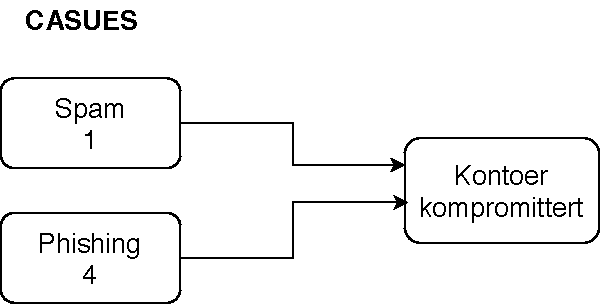
\includegraphics[scale=0.6]{case_2/bilder/kjente_arsaker.pdf}
    \caption[Kjente årsaker til kompromittert konto]{Kjente årsaker til kompromittert konto}
    \label{fig:kjente-arsaker-kompromittert-konto}
\end{figure}

Phishing er en av de få årsakene vi har noe data på, så det er en av årsakene vi vil holde fokus på i analysen. Bildet under viser et eksempel på en phishing e-post som ble sendt til en ansatt ved NTNU.

\begin{figure}[H]%
    \centering
    \subfloat[Forsøk fra November 2017]{{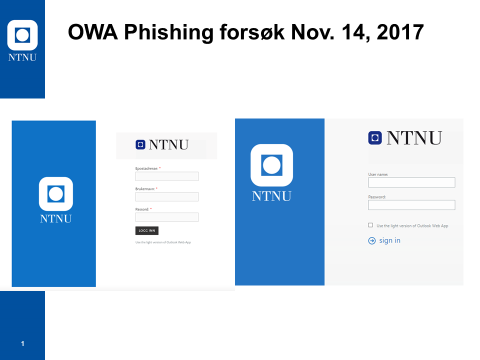
\includegraphics[width=5cm]{case_2/bilder/phishing_1.png} }}%
    \qquad
    \subfloat[Forsøk fra Januar 2018]{{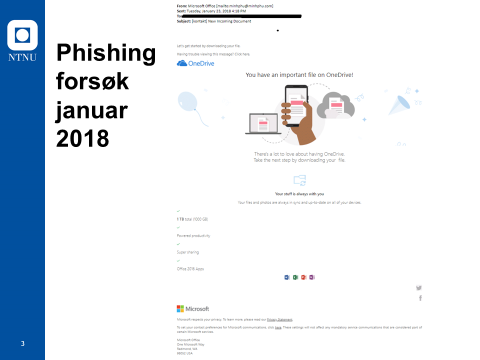
\includegraphics[width=5cm]{case_2/bilder/phishing_2.png} }}%
    \qquad
    \subfloat[Forsøk fra Januar 2018]{{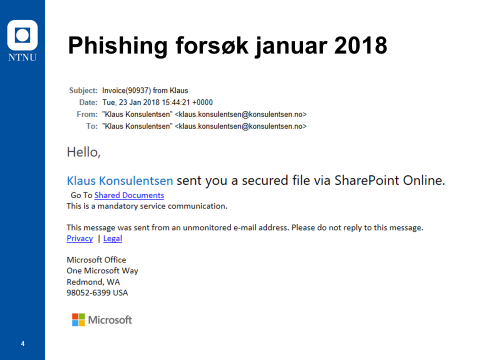
\includegraphics[width=5cm]{case_2/bilder/phishing_3.png} }}%
    \caption{Eksempel på phishing e-post som ble identifisert ved NTNU}%
    \label{fig:example}%
\end{figure}


Universitetet betaler for tilgang til databaser som inneholder tusenvis av forskningsartikler og andre artikler. 26 av de kompromitterte brukerne ble brukt av utenlandske aktører for å skaffe seg tilgang til forskningsartikler. Konsekvensen ved å ha kompromitterte kontoer som laster ned forskningsartikler er ikke bare at NTNU taper penger, men at NTNU risikerer å bli blokkert fra databasene. Angriperne derimot tjener på å ikke trenge å betale for tilgang til databasene. 

Av slike artikler, blir det hentet ut flere tusen på en gang per bruker. Universitetet vet ikke om når det blir hentet ut artikler, eller om det er legitimt bruk av artiklene. De får ofte vite det først når universitetet får beskjed av samarbeidspartnere til NTNU, for eksempel de som tilbyr artiklene. 


Kompromitterte kontoer blir ofte solgt på svartebørsen. 
\begin{figure}[H]
    \centering
    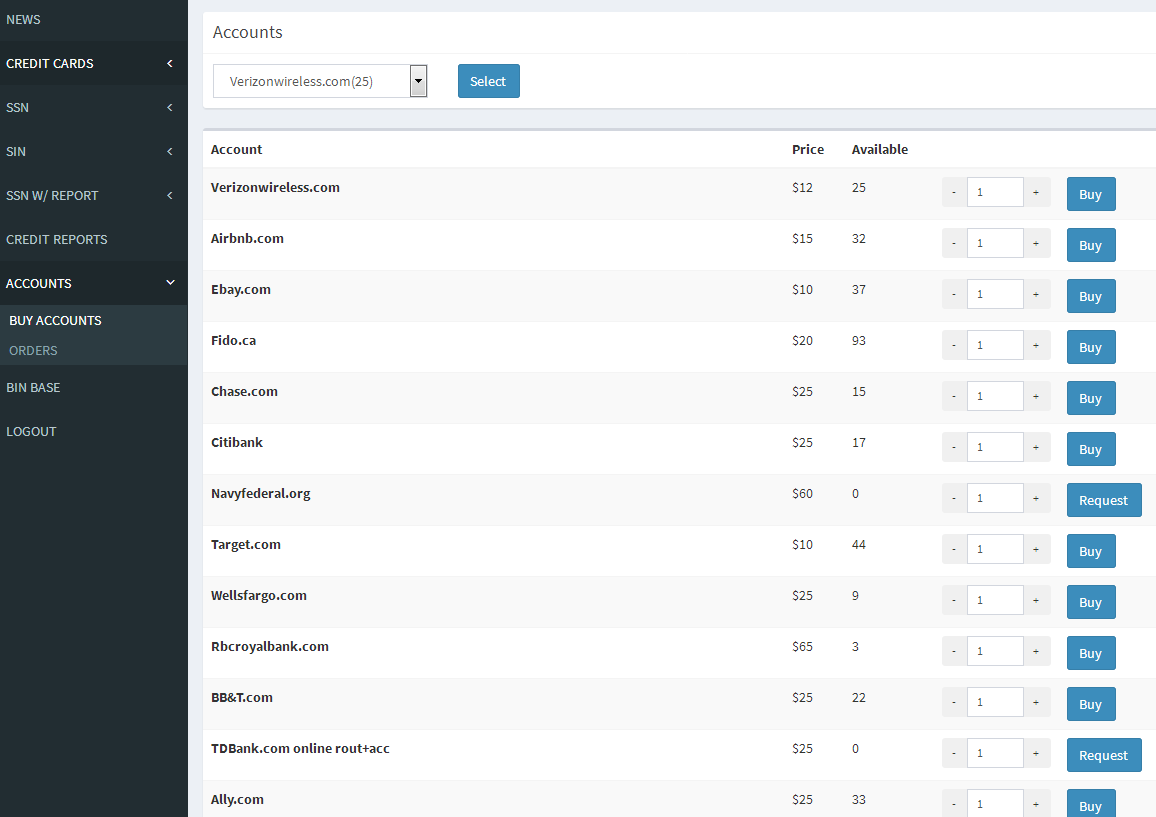
\includegraphics[scale=0.4]{case_2/bilder/prislite_kontore.png}
    \caption[pris-kontoer]{Pris på kontoer}
    \label{fig:pris-kontoer}
\end{figure}
Kilde: https://krebsonsecurity.com/2017/12/the-market-for-stolen-account-credentials/


Dette viser at det er et stort marked for brukerkontoer, og siden NTNU har mange samarbeidspartnere er de et stort mål for trusselaktørene. 


Denne analysen går ut på å identifisere rotårsaken til hvordan NTNU har så mange kompromitterte brukerkontoer, og i løpet av rapporten vil vi svare på følgende forskningsspørsmål:
\begin{itemize}
    \item Hva er rotårsaken til at brukerkontoer ved NTNU blir kompromittert?
    \item Hvordan fungerer rotårsaksanalyse i et case som omhandler misbruk av datakraft?
\end{itemize}


\section{Metode}

Metodebruken i denne analysen er delt inn i syv steg som vist i figur \ref{fig:prosess} under. I hvert steg av denne prosessen brukes det ulike verktøy for å hjelpe til med å forstå problemet, finne rotårsak, og tilslutt implementere tiltak for å eliminere årsakene. Verktøyene fra metoden som blir brukt i hver fase vises til høyre for fasene i figuren under. 
\begin{figure}[H]
    \centering
    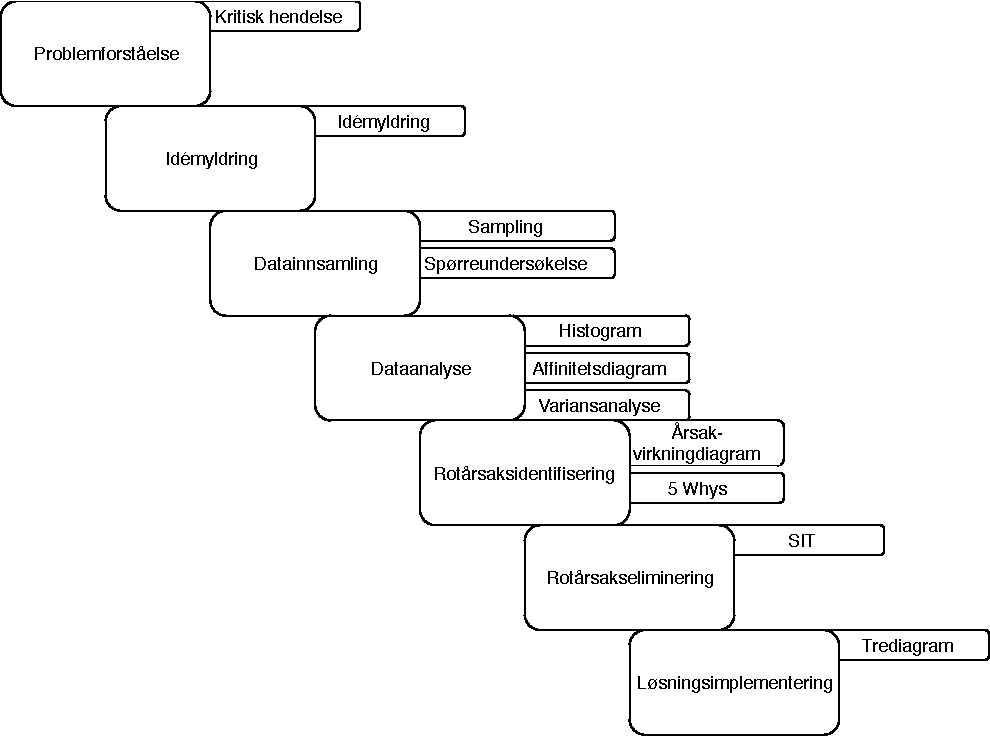
\includegraphics[scale=0.6]{case_2/bilder/RCA-Prosess-case-2.pdf}
    \caption[Rotårsaksanalyseprosessen]{Rotårsaksanalyseprosessen definert av Andersen og Fagerli}
    \label{fig:prosess}
\end{figure}
\chapter{Problemforståelse}
Denne fasen eksisterer for å passe på at en har forstått problemet i dypere detalj. Verktøyene som er relevante å bruke skal gi en bedre forståelse av blant annet omfanget og de ulike aspektene ved et problem. Jo bedre tilgang en har på informasjon, logger og dokumentasjon, jo bedre vil denne fasen kunne utføres. Grunnet god erfaring ved bruk av verktøyet kritiske hendelser i det foregående caset, og på grunn av tilgang på relevant informasjon til bruk i verktøyet, har vi igjen valgt å bruke dette. 


\section{Kritiske hendelser}
For å lære mer om bakgrunnen til problemet bruker vi verktøyet kritiske hendelser for å se på frekvensen av misbruk som er registrert fra de kompromitterte kontoene. Slik kan vi kartlegge og forstå hva de kompromitterte kontoene brukes til. Denne informasjonen ble gitt fra oppdragsgiver.

\subsection{Ønsket utbytte}
Ved bruk av dette verktøyet ønsker vi å få en oversikt over hvilke handlinger de kompromitterte kontoene utfører. Dette går i stor grad ut på hva som er motivasjonen til trusselaktørene. Vi ønsker å danne et bilde av hva de ønsker å oppnå ved å kompromittere kontoene, slik at vi kan bruke den informasjonen senere til å finne rotårsaken til at de blir kompromittert. 

\subsection{Gjennomføring}
Sammen med oppgavebeskrivelsen fikk vi en liste over loggførte sikkerhetshendelser som hadde foregått det siste året hvor kompromitterte kontoer var involvert. Dataene ble sortert i synkende rekkefølge og lagt inn i en tabell for å visualisere frekvensen til de enkelte sikkerhetshendelsene, og dermed fokusområdene til trusselaktørene. 

\subsection{Resultater}
\begin{table} [H]
    \begin{tabular}{ | m{18em} | m{18em} | }
        \hline
            \cellcolor{yellow} Sikkerhetshendelser & \cellcolor{yellow} Frekvens \\
        \hline
            Spam & 46  \\
        \hline
            Misuse (uthenting av forskningsartikler) & 26 \\
        \hline
            Negligible/Fixed/Failed Attack  & 8 \\
        \hline
            Phishing & 7 \\
        \hline
            Whaling & 2 \\
        \hline
            Brute force & 2 \\
        \hline
            DDOS out & 1 \\
        \hline
            Traded credentials & 1 \\
        \hline
            Hackingtools exploits and kits & 1 \\
        \hline
            Copyright/Piracy & 1 \\
        \hline
    \end{tabular}
    \caption{Oversikt over hva kompromitterte ansattkontoer blir brukt til}
    \label{kritisk_tabell_2}
\end{table}

Fra tabellen ser vi at spam er den hendelsen med høyest frekvens, men etter diskusjon med oppdragsgiver var ikke dette problemet av størst viktighet. Det er fordi dette er noe som enkelt blir lagt merke til og er trolig ikke hovedgrunnen til at aktørene aktivt går inn for å kompromittere NTNU sine brukerkontoer. Når det kommer til misuse i tabellen ovenfor referer det til hendelser der uvedkommende misbruker NTNU sine ressurser, spesielt i form av å stjele forskningsartikler på NTNU sin regning. Dette var en av de største problemene med kompromittering av kontoene, siden det førte til økonomisk tap for NTNU og fare for utestengelse fra artikkeldatabasene. 


\subsection{Konklusjon av verktøyet}
I dette caset fungerte metoden godt siden vi hadde all data på forhånd og trengte bare få satt det i system. Verktøyet hjalp veldig til å se hvilke symptomer som er av høyest frekvens. Det negative med verktøyet i dette caset var at det ikke beskriver hvor kritiske enkelthendelsene er, bare hvor mange det er av de. Kritikaliteten til enkelthendelsene måtte vi forhøre oss med oppdragsgiver for å komme fram til. I tabellen vår ser vi at spam ligger på topp, men det viser seg at misuse egentlig er mer kritisk, selv om det ligger under. 





\chapter{Idémyldring}
I dette steget i prosessen er målet å generere en liste over det vi tror kan være mulige årsaker til problemet. Det er en del forskjellige verktøy en kan bruke for å oppnå dette, men vi har valgt å benytte Idémyldring på basis av RCA boken \cite{RCA} sin fremgangsmåte for valg av verktøy, og på bakgrunn av vår tidligere kunnskap om hvordan brukere vanligvis kompromitteres. 

\section{Idémyldring}
I rotårsaksanalyse finnes det to ulike måter å gjennomføre idémyldring på: strukturert- og ustrukturert idémyldring. I den strukturerte versjonen får hver deltaker sin tur til å komme med en idé, og dette sikrer at alle får delta like mye. På den ustrukturerte måten kan alle komme med idéer etterhvert som de kommer på dem, og fungerer mye mer spontant enn den strukturelle. Det er spesielt viktig å ikke omformulere eller diskutere forslagene etterhvert som de kommer, dette skal gjøres etter idémyldringsøkten er over.

\subsection{Ønsket utbytte}
Ønsket utbytte ved å bruke idémyldring var for å få en forståelse av hva som kan være rotårsaken til at ansatte sine kontoer blir kompromittert, og hvordan passord og brukernavn kan komme på avveie.

\subsection{Gjennomførelse}
Det første som ble gjort når økten startet var å kommunisere og skrive opp problemstillingen på en tavle. Vi valgte å organisere idémyldringen som et tankekart ettersom dette var en kjent løsning for gruppen. Den ustrukturerte tilnærmingen til idémyldring ble brukt på grunn av dens uformelle struktur. Ingen er heller dominerende i gruppen, som gjør det mulig for alle å komme med innspill. Hvis noen i gruppen hadde vært dominerende hadde vi heller gått over til å bruke skriftlig idémyldring, også kjent som idéskriving. 

Vi diskuterte og prøvde å komme på mulige måter trusselaktører kan kompromittere brukerkontoer til de ansatte ved universitetet, og hvordan passord og brukernavn kan komme på avveie.

\subsection{Resultater}
Etter øktene var ferdig ble det gjort en vurdering av resultatene og de ble kategorisert i henhold til likhetstrekk, under en fellesnevner som for eksempel sosial manipulering. Resultater og grupperinger er som vist i figur \ref{fig:idemyldring} under.

\begin{figure}[H]
    \centering
    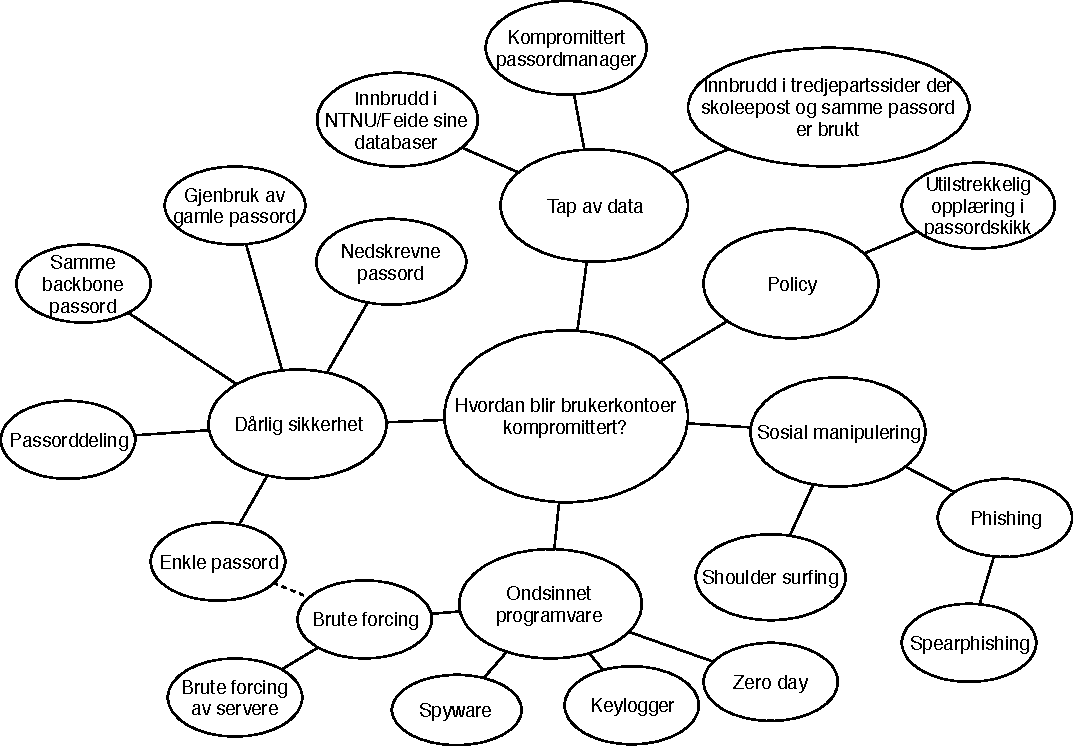
\includegraphics[scale=0.5]{case_2/bilder/idemyldring.pdf}
    \caption[Idémyldring]{Resultater og gruppering av idémyldringen}
    \label{fig:idemyldring}
\end{figure}

Resultatene er gruppert inn i 4 hovedkategorier:
\begin{description}
    \item [Dårlig sikkerhet] er alt fra enkle passord til passordgjenbruk.
    \item [Tap av data] inkluderer at for eksempel sider som dropbox har en lekkasje av brukere.
    \item [Sosial manipulering] vil si å få tak i informasjon ved å lure noen.
    \item [Ondsinnet programvare] er programvare brukt som hjelpemiddel for å få tak i brukerinformasjon.
\end{description}

\subsection{Konklusjon av verktøyet}
Dette var et effektivt verktøy for å få en overordnet oversikt over hva årsakene til at brukerkontoer blir kompromittert og grunner til at passord og brukernavn kan være på avveie. Verktøyet fungerte godt til å komme med mulige måter for aktører å få tilgang til brukerkontoer, eneste som trekker tilbake er det at vi ikke har fått et godt bilde av hvorfor angripere velger å gå etter ansattkontoer, selv om vi fikk et litt simpelt bilde på dette med problemforståelsen.

\chapter{Datainnsamling}
Målet i denne fasen er å samle inn et så bredt aspekt av informasjon som mulig gjennom et par mulige verktøy og teknikker beskrevet i boka om rotårsaksanalyse\cite{RCA}.



%----------------------KVANTITATIVE SPØRREUNDERSØKELSE--------------------------
\section{Elektronisk spørreundersøkelse}
Det finnes i hovedsak to forskjellige undersøkelsestyper, kvantitative og kvalitative spørreundersøkelser. Kvalitative undersøkelser går ut på å spørre få personer, og samle mer detaljerte svar av høyere kvalitet, gjerne langsvar. Kvantitative undersøkelser fungerer motsatt i at det er fokus på mange tilbakemeldinger slik at en kan senke usikkerhet knyttet til svarkvalitet og gjøre statistisk analyse på resultatene. I vår undersøkelse har vi i hovedsak valgt å fokusere på en kvantitativ spørreundersøkelse, med noen få kvalitative elementer. 

Grunnen til at vi valgte i hovedsak kvantitativ spørreundersøkelse er at vi ønsker å finne relasjoner mellom dataene vi samler inn. Det er også mulighet for å gjøre statistiske beregninger på disse, noe vi anser som relevant for datainnsamlingen i dette caset. Fremstilling av data i grafer og tabeller er også et moment som gjorde at valget ble kvantitativ metode. 

\subsection{Ønsket utbytte}
Med den elektroniske spørreundersøkelsen ønsker vi å få informasjon fra personer som allerede har fått brukeren sin kompromittert. Informasjonen vil bestå av blant annet personens passordvaner, kjennskap til retningslinjer om passordbruk og epost-aktivitet. Vi håper å få minst 30 respondenter, som vil være akkurat nok for en kvalitativ analyse. 

\subsection{Gjennomføring}
Under idémyldringen ble det avdekket en rekke faktorer som kunne være medvirkende i at ansatte og studenter ved NTNU fikk sin konto på avveie. Vi brukte denne informasjonen aktivt da spørreundersøkelsen ble konstruert. Spørreundersøkelsen slik den fremstår for respondenten finnes i vedlegg \ref{undersokelse_norsk}. Med spørreundersøkelsen ble det sendt med en liten tekst for å oppmuntre de til å ta den. Her ble det brukt mye patos ettesom dette er et ømfintlig tema. For nesten hvert spørsmål ble en tilhørende hypotese bestemt. I tabell \ref{tab:hypoteser} under har vi listet opp hypotesene til de tilhørende spørsmålene.


% Table generated by Excel2LaTeX from sheet 'Ark2'
\begin{table}[H]
  \centering
  \caption{Hypoteser til spørsmålene}
    \begin{tabular}{|p{20.215em}|p{20.57em}|}
    \hline
    \rowcolor{yellow} Spørsmål & Hypoteser \\
    \hline
    Din alder? & Eldre er overrepresentert i statistikken over tapte kontoer \\
    \hline
    Ditt kjønn? & Flere kvinner enn menn har blitt kompromittert \\
    \hline
    Hva er din primærrolle ved NTNU? & Det er ansatte som er målgruppen til trusselaktørene \\
    \hline
    I hvilken by jobber/studerer du primært? & Gjøvik har høyere sikkerhetskompetanse \\
    \hline
    I hvor mange år har du jobbet/studert ved NTNU eller de tidligere høgskolene? & Folk med lavere ansiennitet kjenner universitetets retningslinjer bedre \\
    \hline
    Når fant du ut at NTNU kontoen din var blitt kompromittert? & Folk vet ikke at de har blitt kompromittert før de blir kontaktet \\
    \hline
    Har du noen formening om hvor lang tid kontoen var kompromittert før Seksjon for Digital Sikkerhet kontaktet deg? & Ingen hypotese grunnet vagt spørsmål \\
    \hline
    Har du noen formening om hvordan kontoen din ble kompromittert? & Ingen hypotese grunnet åpent svar \\
    \hline
    Bruker du din NTNU e-post til å registrere deg på ulike tjenester på nett i forbindelse med jobben/studiet? & Over halvparten bruker NTNU e-post til tjenester i forbindelse med jobb \\
    \hline
    Bruker du din NTNU e-post til å registrere deg på tjenester på nett til privat bruk? & Under halvparten bruker NTNU e-post til privat bruk \\
    \hline
    På en skala fra 1-6, der 1 er lite bevisst og 6 er svært bevisst, hvor bevisst er du på sikkerhet når du... & \multirow{4}[2]{*}{Folk er generelt sett lite bevisste} \\
    besøker nettsider? & \multicolumn{1}{r|}{} \\
    lager passord? & \multicolumn{1}{r|}{} \\
    sjekker e-post? & \multicolumn{1}{r|}{} \\
    \hline
    Har du i din tid hos NTNU lagt merke til phishing-forsøk mot deg på din NTNU e-post? & Phishing er en svært utbredt angrepsvektor \\
    \hline
    Har du blitt lurt av phishing på din NTNU e-post? & Av de som har blitt kompromittert har under en tredjedel blitt lurt av phishing \\
    \hline
    Har du i løpet av din tid ved NTNU eller de andre høgskolene, oppdaget virus eller annen skadevare på maskinen din? & Virus og annen skadevare er utbredt \\
    \hline
    Bruker du ditt NTNU passord på flere tjenester? & Passordgjenbruk er utbredt \\
    \hline
    Brukte du regler til å generere ditt NTNU passord? & De fleste bruker ikke passordregler til å generere passord \\
    \hline
    Er ditt NTNU passord tilfeldig sammensatt av bokstaver, tall og/eller tegn? & De fleste bruker ikke tilfeldig sammensatte passord \\
    \hline
    Hvor mange tegn består ditt NTNU passord av? & Over halvparten har passord på under 12 tegn \\
    \hline
    Har du i løpet av din tid ved NTNU delt NTNU passordet ditt med andre? & Passorddeling er ikke særlig utbredt \\
    \hline
    Omtrent hvor ofte bytter du ditt NTNU passord? & Passord byttes for det meste sjeldnere enn hvert andre år \\
    \hline
    Bruker du en passordmanager? & De fleste bruker ikke passordmanager, og mange vet ikke engang hva det er \\
    \hline
    På en skala fra 1 til 6, hvor godt kjent er du med... & \multirow{4}[2]{*}{Det er svært lite kjennskap til retningslinjer} \\
    NTNU sine retningslinjer for behandling av brukernavn, passord og andre autentiseringsdata? & \multicolumn{1}{r|}{} \\
    IT reglementet til NTNU? & \multicolumn{1}{r|}{} \\
    NTNU sine prinsipper for informasjonssikkerhet? & \multicolumn{1}{r|}{} \\
    \hline
    Har du fått opplæring i passordsikkerhet fra NTNU? & Under en fjerdedel har fått opplæring i passordskikk fra NTNU \\
    \hline
    \end{tabular}%
  \label{tab:hypoteser}%
\end{table}%

Undersøkelsen var kvalitetskontrollert flere ganger av forskjellige personer, inkludert medstudenter, veileder og ikke minst oppdragsgiver. Undersøkelsen ble laget i SelectSurvey, med tilhørende NTNU tema for utformingen. Dette ble gjort for å få spørreundersøkelsen til å virke legitim, siden den har NTNU sin logo i hjørnet og nettadressen tilhører NTNU sitt domene. 

Spørreundersøkelsen ble sendt ut til totalt 167 personer, men den nådde bare 157 av e-post addressene. Alle disse hadde fått sin NTNU konto kompromittert i tidsperioden 1. November 2016 til 1. April 2018. E-post listen ble opprettet av oppdragsgiver basert på intern data og sent ut på vegne av Seksjon for Digital Sikkerhet. 

Det ble oppdaget et par småfeil i spørreundersøkelsen etter den var utsendt. Blant annet var det glemt et ``vet ikke'' alternativ på spørsmålet om de hadde en formening om hvor lang tid det hadde gått fra kompromittering til de fikk beskjed. Dette fikk vi fikset ved å legge til tekst om at du kunne la det være blankt om du ikke visste, slik at det ikke gikk altfor mye ut over svarene, og spørsmålet ble endret til å ikke være obligatorisk. Det var også glemt en kommentarboks helt i slutten av spørreundersøkelsen, som vi bestemte at vi ikke kunne plassere inn etter den var utsendt. Det var også et par småfeil i formulering, men dette fikk vi endret underveis. Endringene ble gjort på natten da vi antok ingen svarte. 

\subsection{Resultater}
Av de som e-posten ble sendt ut til fikk vi totalt 72 gyldige respondenter, mens 26 stoppet rett etter åpning av undersøkelsen eller underveis. Undersøkelsen var aktiv i perioden fra 20. April til og med 27. April. I løpet av denne tiden ble det sendt ut én purring den 25. April. 

\subsection{Konklusjon av verktøy}
Dersom en feil er stor i en spørreundersøkelse kan ikke denne rettes opp i underveis. Dette er en av svakhetene med denne typen datainnsamling. Det kan i værste fall få konsekvenser for datasettet. Heldigvis var det ikke kritisk for oss, og vi fikk rettet opp det meste. Det positive var at vi hadde håpet på litt over 30 svar, men endte opp med 72, som var omtrent 45\% av de som mottok e-posten. Kanskje det var bruken av patos i e-post og innledning, i tillegg til at dette var et relevant tema for dem, som førte til høy svarprosent. 

\chapter{Dataanalyse}
I denne fasen analyseres dataene som er samlet inn, og ved hjelp av statistiske verktøy kan vi trekke konklusjoner basert på svarene. I analysen kommer vi hovedsaklig til å bruke verktøy som er beskrevet i metodeboken \cite{RCA}, men vi har også benyttet oss av statistiske verktøy som kan gå dypere, men som ikke er like visuellt fremstillende. Etter denne fasen ønsker vi å sitte igjen med en mengde mulige årsaker til at NTNU sine kontoer blir kompromittert. Verktøyet vi har brukt til å utføre mesteparten av analysene er SPSS, et statistisk verktøy for å blant annet gjøre grafiske- og matematiske beregninger på et datasett.

\section{Ønsket utbytte}
Her beskrives det ønskede utbytte av de forskjellige verktøyene som er benyttet i analysefasen og hva vi bruker de til.

\subsection{Histogram}
Ved å benytte histogram håper vi å få en visuell fremstilling av data som gjør det raskt og enkelt å forstå disse, og derfor lettere kunne trekke konklusjoner. Disse blir stort sett brukt for å få en oversikt over svarprosent på enkeltsspørsmål. 

\subsection{Sektordiagram}
Med et sektordiagram ønsker vi å fremstille fordelingen i demografien der det er få kategorier. 

\subsection{Affinitetsdiagram}
Et av spørsmålene i spørreundersøkelsen var et kortsvar der respondentene selv kunne komme med sin formening om hvordan kontoen deres ble kompromittert. Ved å bruke affinitetsdiagram håper vi på å få samlet og gruppert disse dataene slik at vi kan se om noe blir sagt flere ganger, og kan være en mulig årsak. 

\subsection{Statistiske analyseverktøy}
Ved å bruke statistiske analyseverktøy som ANOVA og Independent-samples t-test ønskes det å finne tilsynelatende skjulte relasjoner eller forskjeller mellom demografien og kjennskap til retningslinjer, bevissthet på sikkerhet og e-post og passordvaner. Vi ønsker også å se om det er noen relasjoner mellom andre spørsmål. ANOVA ble brukt dersom den uavhengige variabelen består av mer enn to grupper. Dersom den bestod av to grupper ble Independent t-test heller brukt.

\section{Svarstatistikk}
Spørreundersøkelsen ble mottatt av 157 personer som har fått kontoen kompromittert. Av disse var det 72 som svarte. Det var i tillegg 26 som startet spørreundersøkelsen, men ikke fullførte. 

Tabellen under viser statistikk over hvor mange svar som kom inn per dag. Det var tydelig mest svar dagen spørreundersøkelsen ble lansert, og 25. April, hvor vi sendte ut en purre e-post. 
\begin{figure}[H]
    \centering
    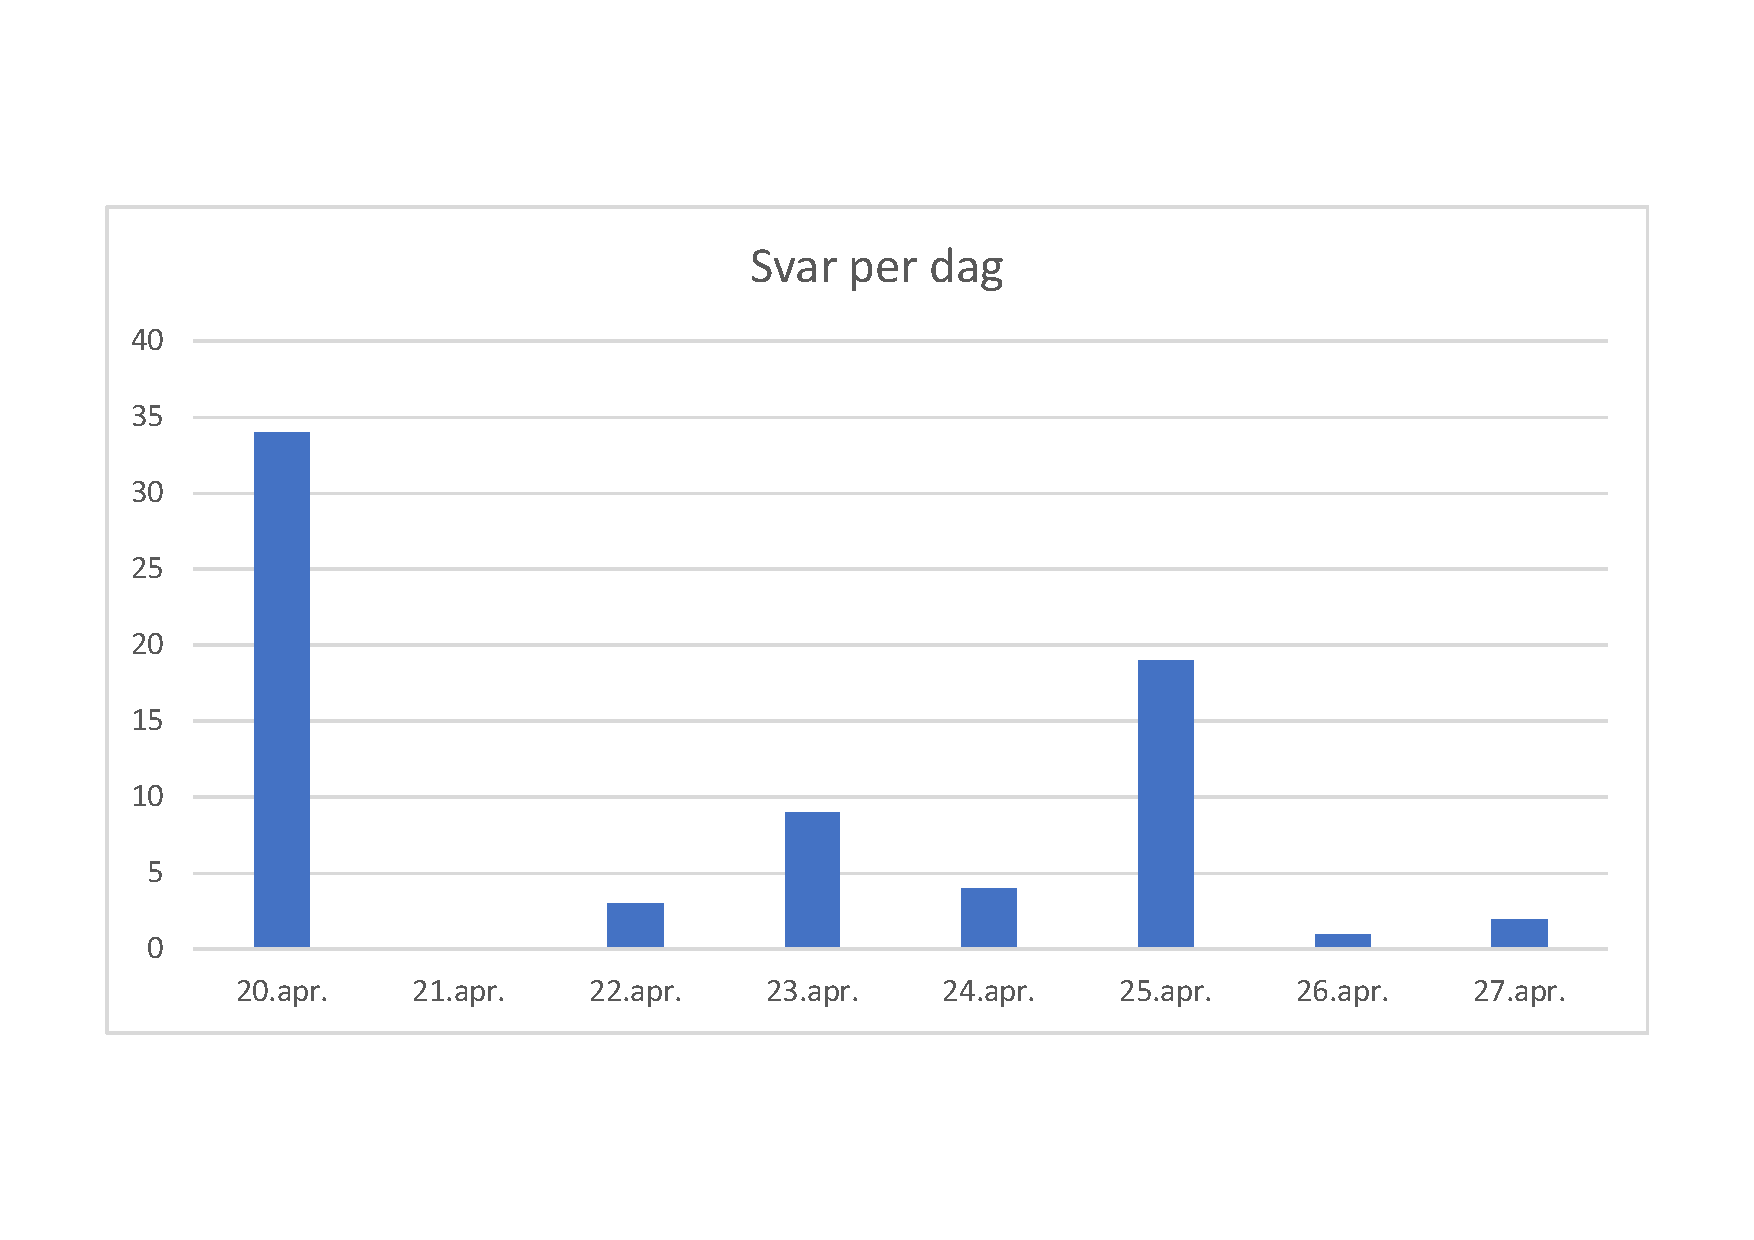
\includegraphics[scale=0.5, clip, trim=1cm 3cm 0cm 3cm]{case_2/bilder/spss/svar_per_dag.pdf}
    \caption[Svar per dag]{Antall svar vi fikk per dag}
    \label{fig:boks}
\end{figure}


%---------------------------------------- DEMOGRAFI ---------------------------------
\section{Demografi}
I denne delen fremlegges resultatene fra demografien i spørreundersøkelsen. Disse blir om mulig sammenliknet med generelle tall fra NTNU for å få et innblikk i demografien til de som har blitt kompromittert kontra NTNU sine ansatte og studenter generelt. Vi fokuserer stort sett på de ansatte siden antall studenter i undersøkelsen var få.

\subsection{Aldersgruppe}
Aldersgruppene ble kategorisert i intervaller på 10 år. Fra de ulike kategoriene fikk vi:

\begin{itemize}
    \item Under 20: 1 person
    \item 20-29: 3 personer
    \item 30-39: 13 personer
    \item 40-49: 27 personer
    \item 50-59: 11 personer
    \item 60-69: 9 personer
    \item 70 eller over: 8 personer
\end{itemize}

Under ser vi aldersfordelingen visuelt fremstilt i et histogram.

\begin{figure}[H]
    \centering
    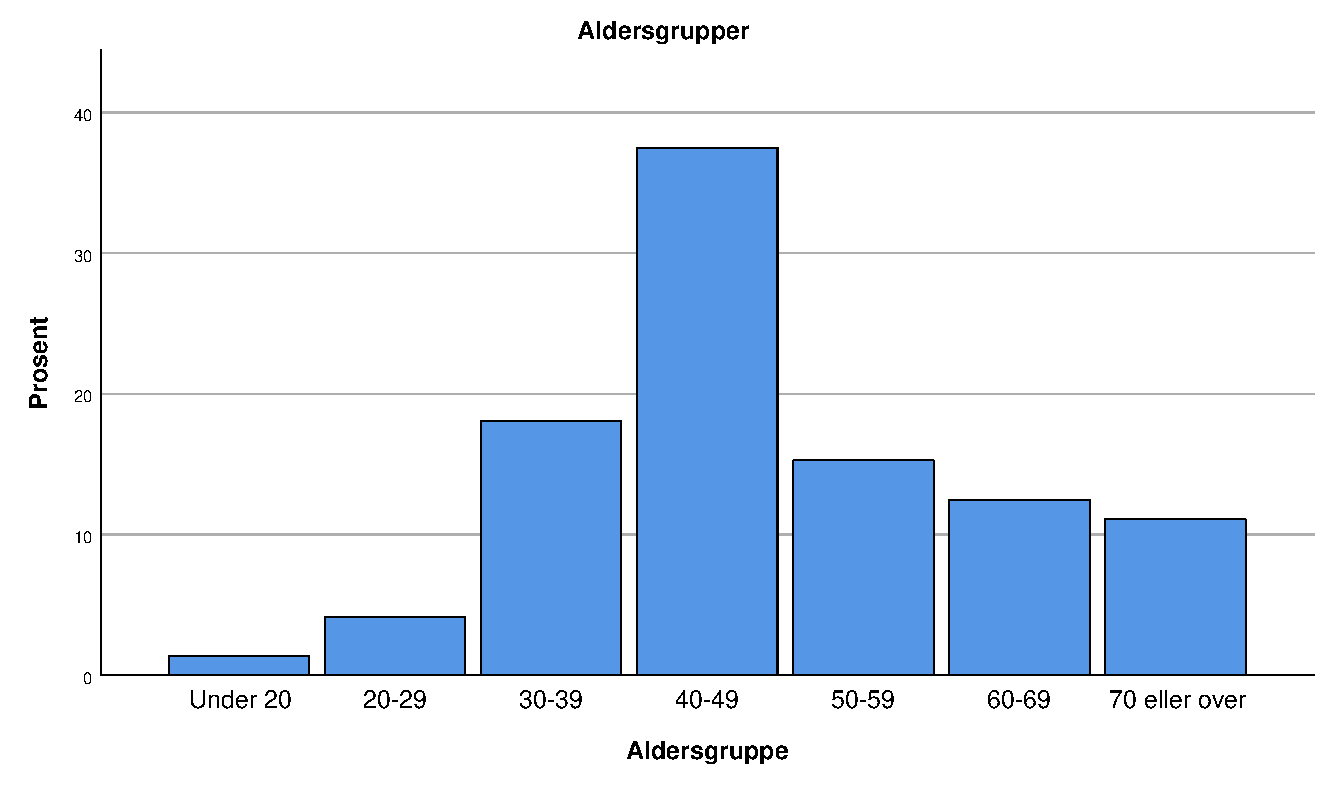
\includegraphics[scale=0.5]{case_2/bilder/spss/aldersgrupper.pdf}
    \label{fig:aldersgruppe}
    \caption[aldersgruppe]{Aldersgrupper av respondentene}
\end{figure}

Ut fra resultatene kan vi konkludere med at de som har blitt kompromittert er stort sett middelaldrene til eldre personer. Disse personene er også noe eldre enn gjennomsnittsalderen til de som jobber ved NTNU \cite{}. SETT INN KILDE: MØRKETALLSUNDERSØKELSE

\subsection{Kjønn}
I spørreundersøkelsen kunne du velge å ikke oppgi kjønn, men dette alternativet var det ingen som benyttet seg av. Av de 72 respondentene var det 45 kvinner og 27 menn. Det er henholdsvis 62,5\% og 37,5\%. Under er kjønnsfordelingen visualisert i et sektordiagram.

\begin{figure}[H]
    \centering
    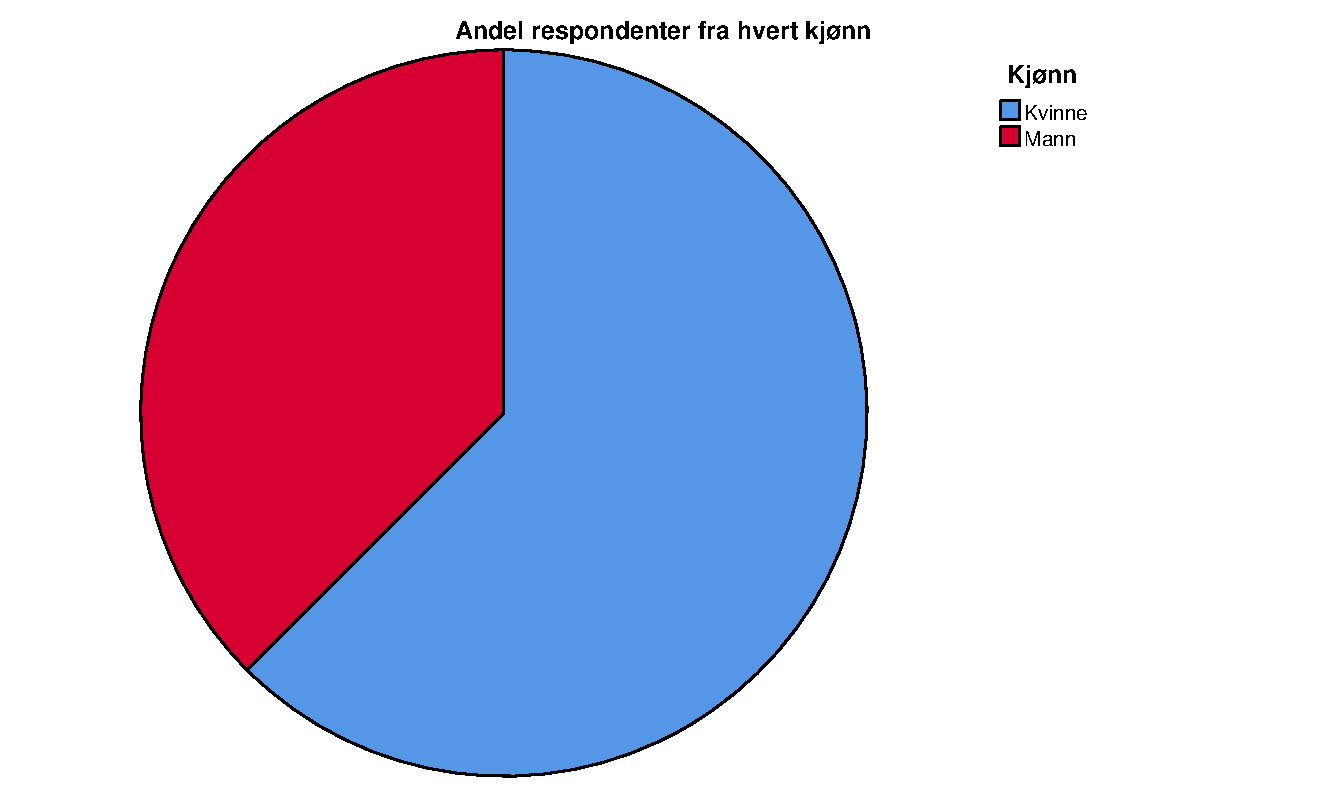
\includegraphics[scale=0.5]{case_2/bilder/spss/kjonn.pdf}
    \label{fig:kjonn}
    \caption[kjonn]{Andel fra hvert kjønn}
\end{figure}

De fleste av de som har svart er kvinner. Av de ansatte ved NTNU er det 41\% kvinner totalt \cite{NTNUfakta}. Totalt sendte vi ut spørreundersøkelsen til 167 e-postadresser, der 157 av de mottok. Vi har tall på at 91 av de 167 vi først sendte ut til var kvinner. Dette er omtrent 55\%. For å kunne si noe om antallet kvinner som svarte på spørreundersøkelsen må vi se på om svarene våre er representative for hele samplet. Vi brukte en kalkulator for å regne ut konfidensintervallet for vårt sample \cite{SSCalc}. Utregningen kom fram til at vi er 95\% sikre på at feilmarginen for dette spørsmålet er \(\pm 8,5\%\). I og med at andelen kvinner totalt på NTNU er 41\%, kan vi fastslå at kvinner er noe mer utsatt for å kontoen kompromittert, men denne forskjellen er ikke stor. 

\subsection{Primærrolle}
Det ble definert to primærroller for å skille mellom ansatte og studenter. Dette ble gjort fordi oppdragsgiver hadde info på at det både var studenter og ansatte som hadde blitt kompromittert. Av de 72 respondentene var det 6 studenter og 66 ansatte. Dette er henholdsvis 8,3\% og 91,7\%. Sektordiagrammet under viser fordelingen. 

\begin{figure}[H]
    \centering
    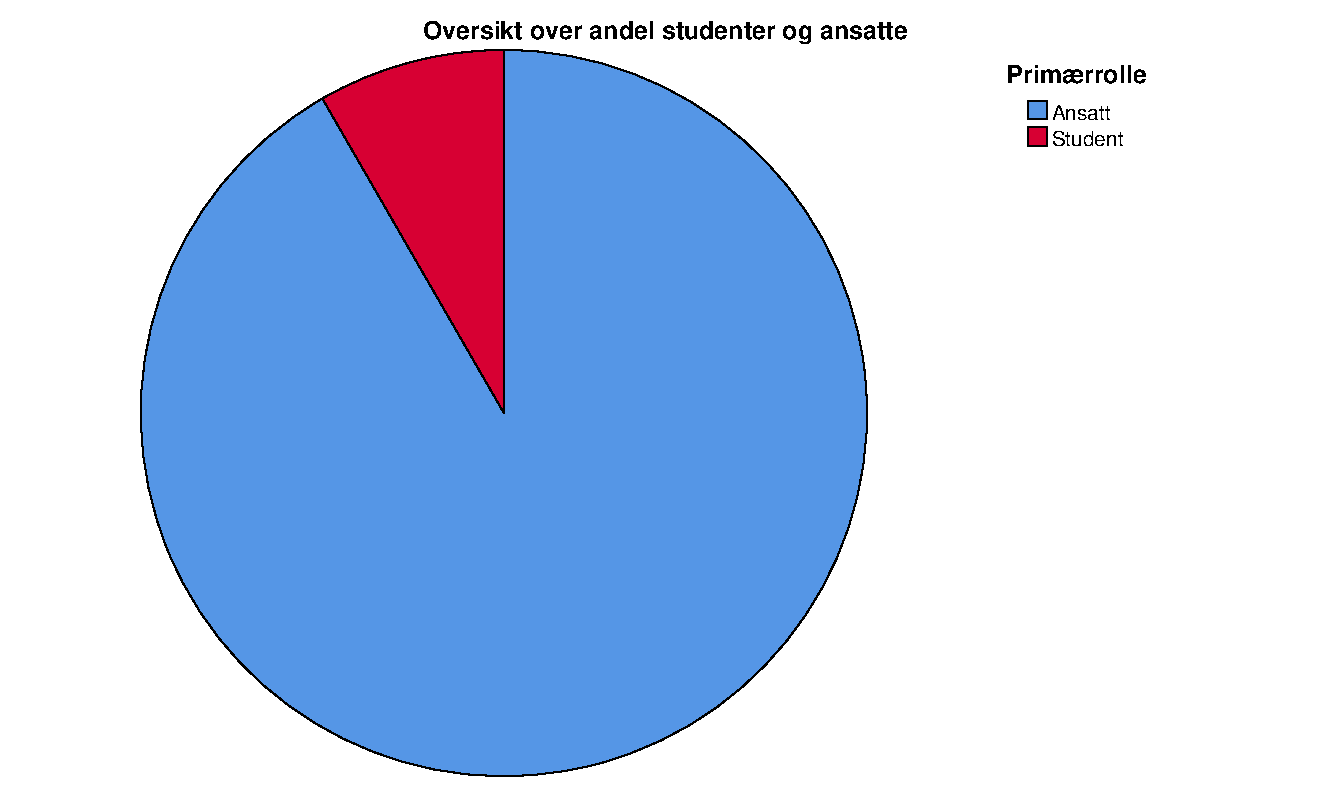
\includegraphics[scale=0.5]{case_2/bilder/spss/primaerrolle.pdf}
    \label{fig:primaerrolle}
    \caption[primaerrolle]{Primærrolle ved NTNU}
\end{figure}

Fra dataene kan vi se at ansatte er overrepresentert i de som blir kompromittert. Vi har data på at det er 18 studenter i vårt sample, altså står studenter for omtrent 10\% av de kompromitterte. På samme måte som i forrige seksjon, ble konfidensintervallet regnet ut \cite{SSCalc}. Utregningen kom frem til at vi er 95\% sikre på at feilmarginen er på \(\pm 5,12\%\). Derfor kan vi med rimelig sikkerhet si at trusselaktørenes målgruppe er de ansatte og ikke studenter. 

\subsection{Primærby}
Av de 72 respondentene var det bare en fra Ålesund og resten var fra Trondheim. Det var ingen respondenter fra Gjøvik. 

\subsection{År ved NTNU}
Bare 6 personer, eller 8,3\% av respondentene hadde jobbet eller studert ved NTNU i under 2 år og i 2 til 4 år. 9 personer, eller 12,5\% hadde jobbet eller studert her i 5 til 9 år, og 15 personer, eller 20,8\% hadde jobbet eller studert her i 10 til 15 år. Hele 36 personer, eller akkurat halvparten av respondentene har vært hos NTNU i over 15 år. En oversikt over disse tallene finnes i histogrammet under. 

\begin{figure}[H]
    \centering
    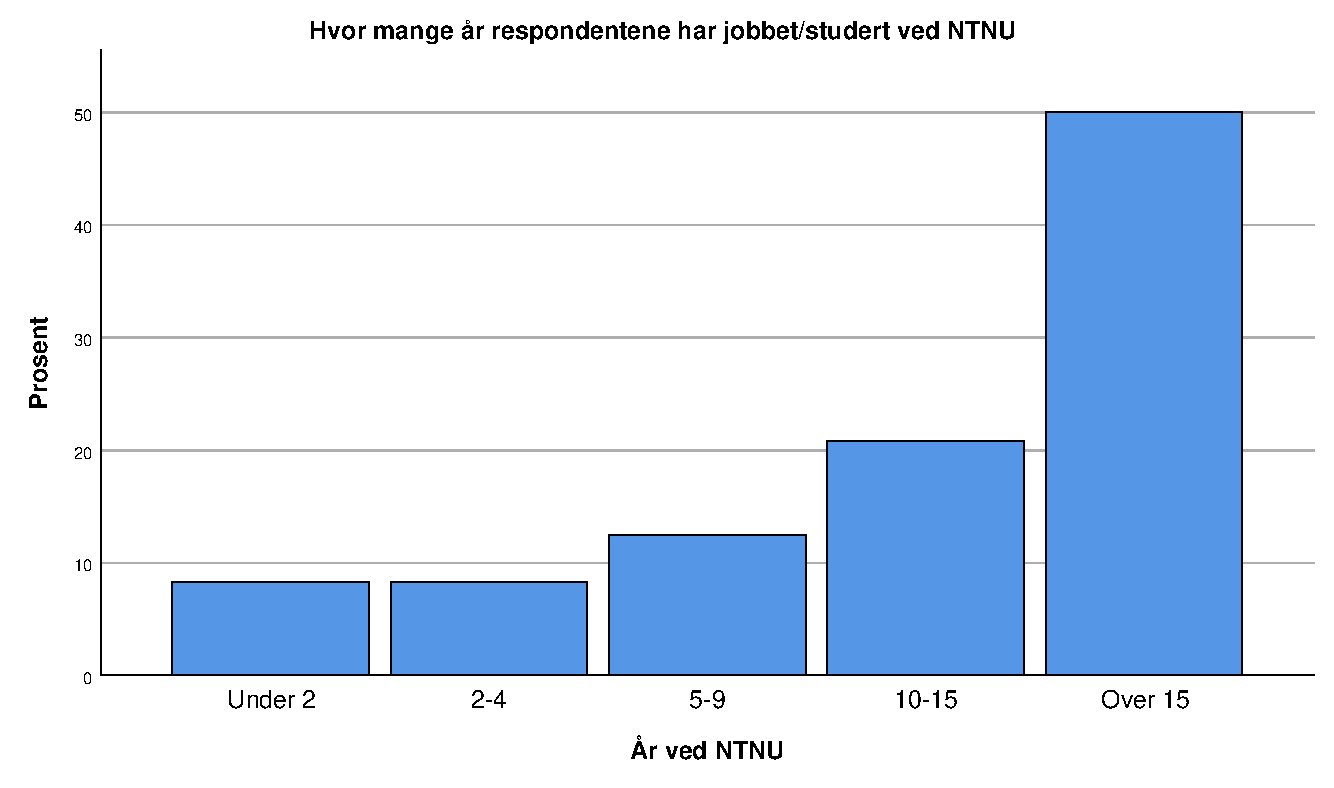
\includegraphics[scale=0.5]{case_2/bilder/spss/aarvedNTNU.pdf}
    \label{fig:aarvedNTNU}
    \caption[aarvedNTNU]{Antall år ved NTNU}
\end{figure}


\subsection{Konklusjon}

%---------------------------------------BEVISSTHET PÅ SIKKERHET---------------------------------
\section{Bevissthet på sikkerhet}
Spørsmålene skulle gi svar på hvor sikkerhetsbevisst en tenker når man besøker nettsider, lager passord og sjekker e-post. Hypotesen som ble fremhevet her var at folk generelt sett er lite bevisste. 

Histogrammet i figur \ref{fig:bevisst-nettsider} viser en tilnærmet normalfordelt situasjon, men med noe fler svar på høyresiden. De fleste er derfor litt mer bevisste på sikkerhet når de besøker nettsider enn de er ubevisste. 
\begin{figure}[H]
    \centering
    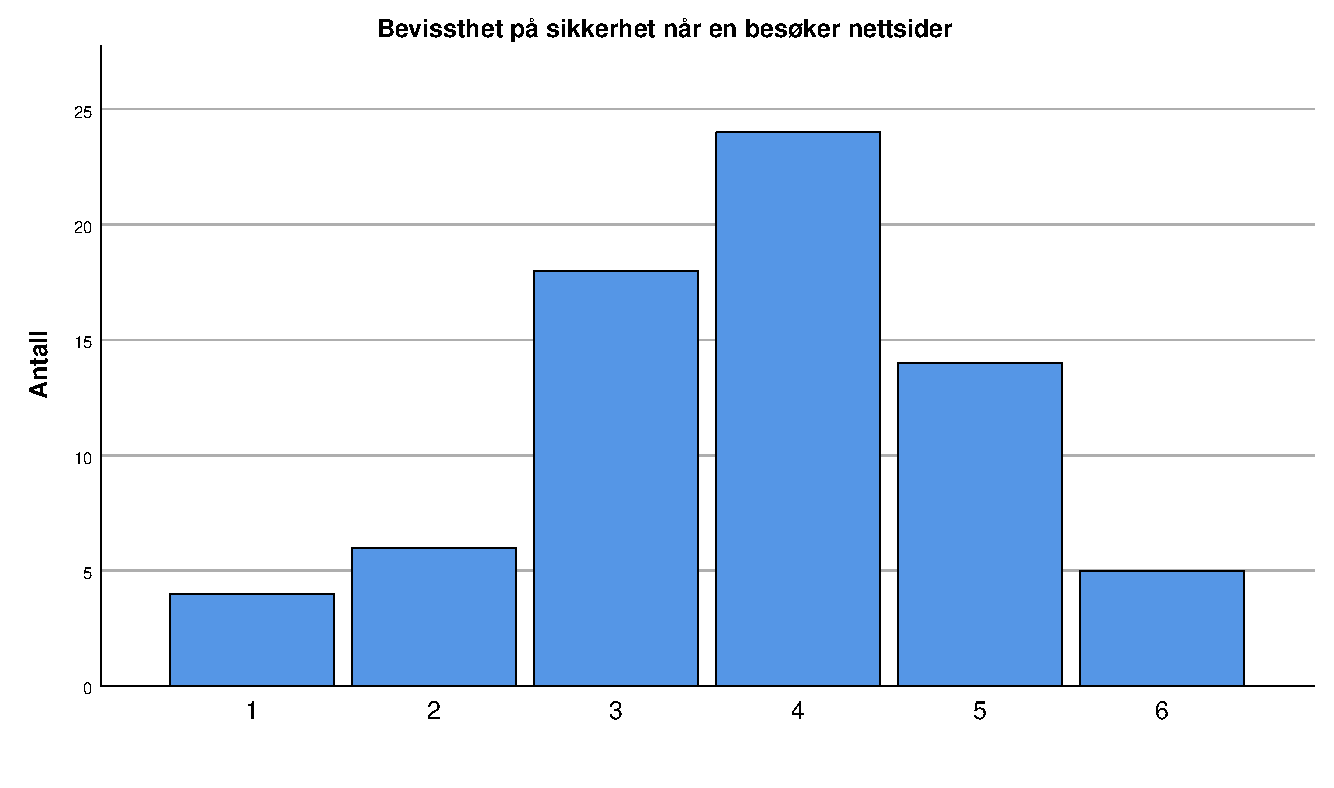
\includegraphics[scale=0.5]{case_2/bilder/spss/bevisst_nettsider.pdf}
    \caption[bevisst-nettsider]{Bevissthet på sikkerhet når en besøker nettsider}
    \label{fig:bevisst-nettsider}
\end{figure}

Når det kommer til sikkerhet når en lager passord svarer respondentene at de generelt sett er bevisste på dette. Figur \ref{fig:bevisst-passord} under viser at fordelingen er konsentrert hovedsaklig på høyresiden.
\begin{figure}[H]
    \centering
    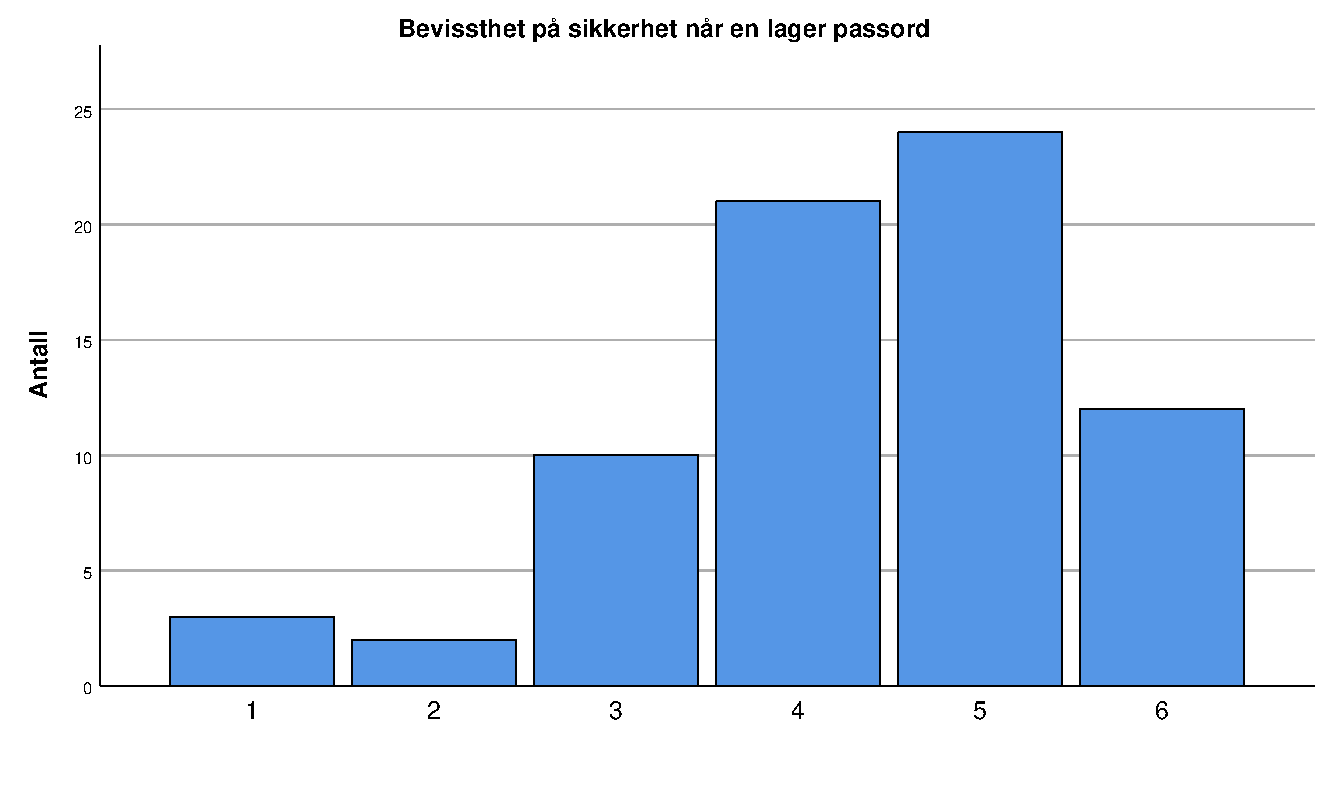
\includegraphics[scale=0.5]{case_2/bilder/spss/bevisst_passord.pdf}
    \caption[bevisst-passord]{Bevissthet på sikkerhet når en lager passord}
    \label{fig:bevisst-passord}
\end{figure}

Figur \ref{fig:bevisst-e-post} under viser bevissthetsfordelingen når det kommer til sjekking av e-post. Dette var noe vi spesielt ønsket å se på siden en av hovedhypotesene våre til kompromitterte brukerkontoer er phishing. Histogrammet viser at respondentene stort sett er bevisste på sikkerhet når de sjekker e-post.
\begin{figure}[H]
    \centering
    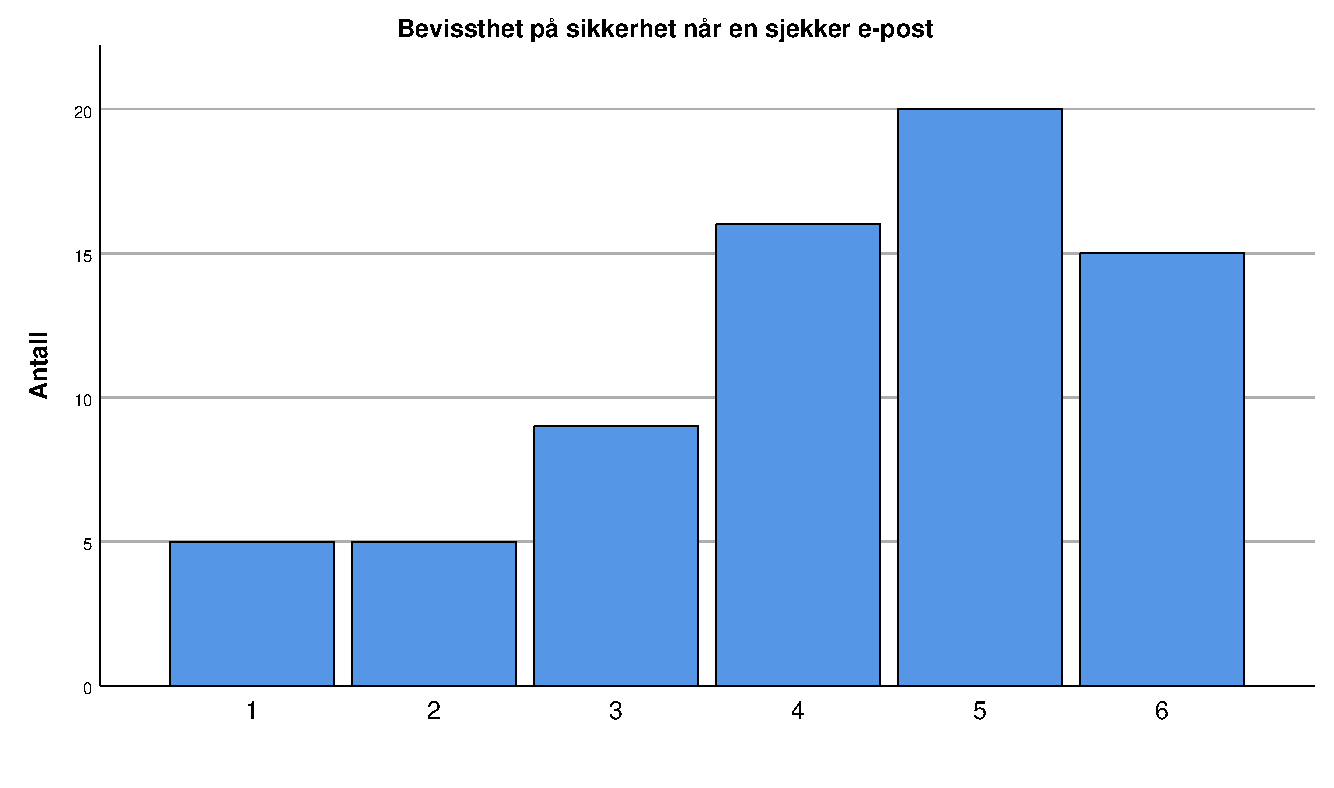
\includegraphics[scale=0.5]{case_2/bilder/spss/bevisst_e-post.pdf}
    \caption[bevisst-e-post]{Bevissthet på sikkerhet når en sjekker e-post}
    \label{fig:bevisst-e-post}
\end{figure}

\subsection{Konklusjon}
Det viser seg at hypotesen vår ikke stemte helt. Vi tror derimot at denne bevisstheten ikke er nok, eller til og med mangelfull. Vi har grunn til å tro at respondentene overvurderer sin egen bevissthet og kompetanse, basert på resten av svarene i denne spørreundersøkelsen. I etterkant har det blitt reist spørsmål rundt validiteten til disse spørsmålene, fordi det spørres om hvor bevisste de er nå, og ikke før de ble kompromittert. Enkelte har gitt tilbakemelding om at de har endret sine rutiner og blitt mer bevisst på sikkerhet i etterkant. Derfor er det grunn til å mene at vi burde spesifisert i spørsmålene hvor bevisste de var før de ble kompromittert.
%---------------------------------------KJENNSKAP RETNINGSLINJER REGLEMENT OG PRINSIPPER---------------------------------
\section{Kjennskap til retningslinjer, reglementer og prinsipper}
Disse spørsmålene handler om hvor godt kjennskap respondentene har til NTNU sine retningslinjer for behandling av autentiseringsdata, IT reglementet og prinsipper for informasjonssikkerhet. Hypotesen vi hadde her var at de aller fleste hadde lite kjennskap til disse.

Det viser seg fra figur \ref{fig:retningslinjer} at respondentene kan lite om NTNU sine retningslinjer for behandling av brukernavn, passord og andre autentiseringsdata. 
\begin{figure}[H]
    \centering
    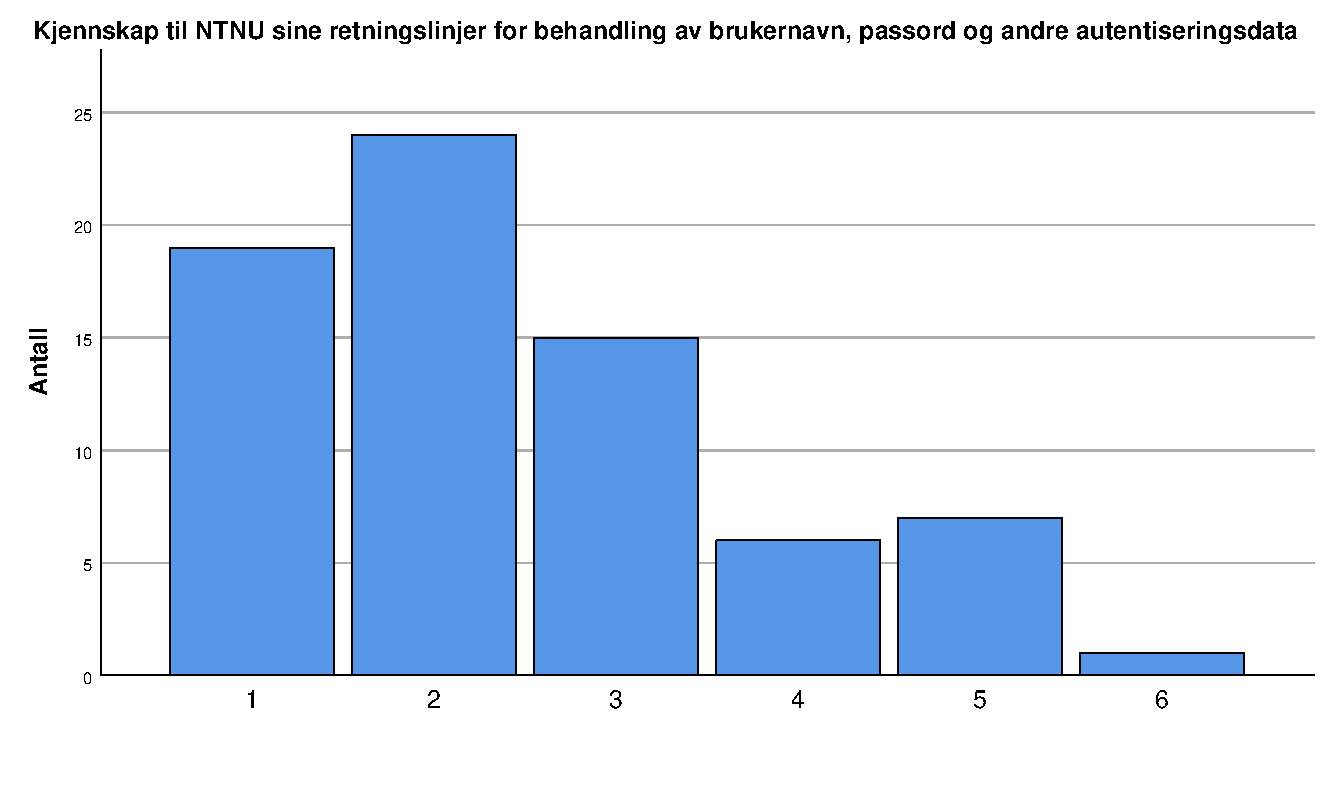
\includegraphics[scale=0.5]{case_2/bilder/spss/retningslinjer.pdf}
    \caption[retningslinjer]{Kjennskap til retningslinjer}
    \label{fig:retningslinjer}
\end{figure}

Figur \ref{fig:ITreglement} viser at respondentene ikke kjenner så godt til IT reglementet til NTNU. Over 70\% svarte tre eller under på hvor godt de kjente IT reglementet til NTNU, der 1 var lite kjent og 6 var meget kjent.  
\begin{figure}[H]
    \centering
    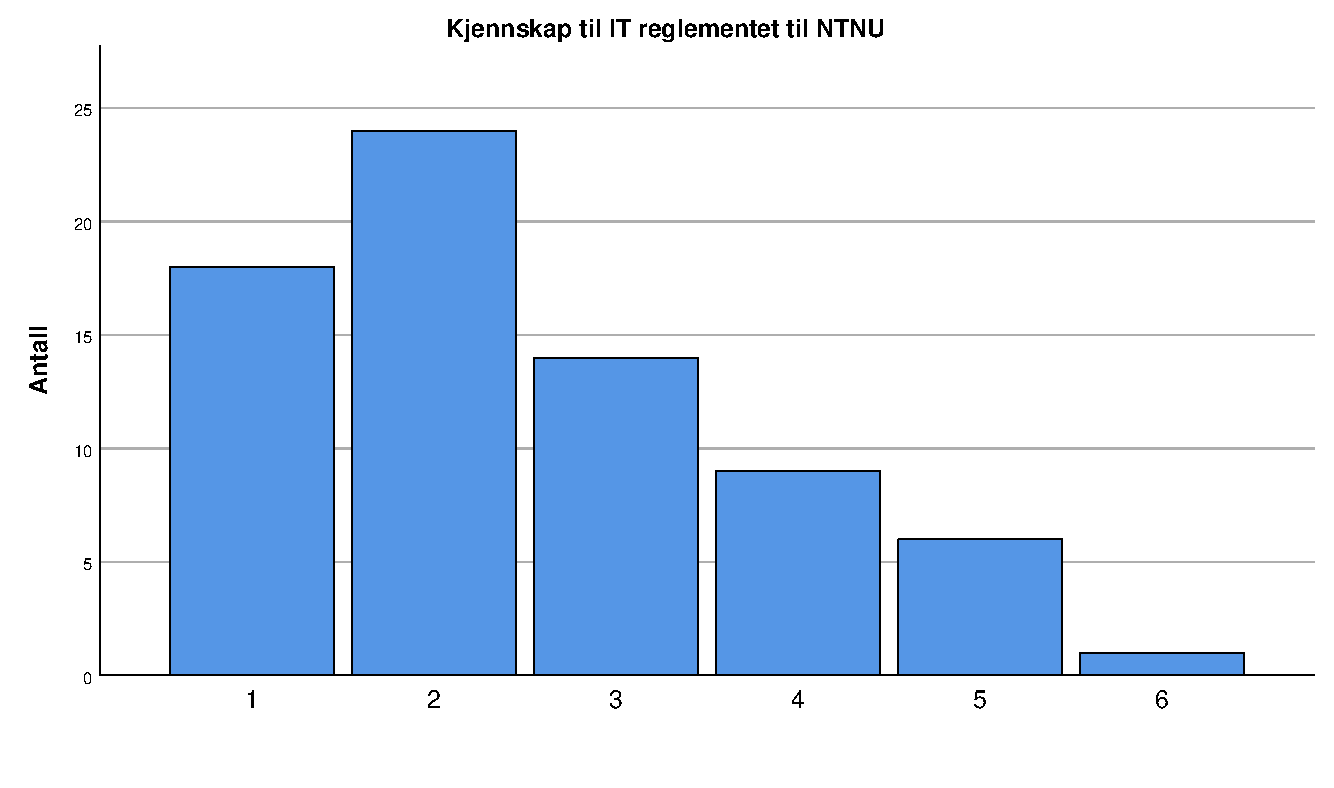
\includegraphics[scale=0.5]{case_2/bilder/spss/ITreglement.pdf}
    \label{fig:ITreglement}
    \caption[ITreglement]{Kjennskap til IT reglement}
\end{figure}

Under viser figur \ref{fig:InfoSecPolicy} at folk har dårlig kjennskap til NTNU sine prinsipper for informasjonssikkerhet. Der står det blant annet at brukere er ansvarlige for enhver bruk av innloggingskredentialier og at de holder dette konfidensielt \cite{PrinsInfoSec}. 
\begin{figure}[H]
    \centering
    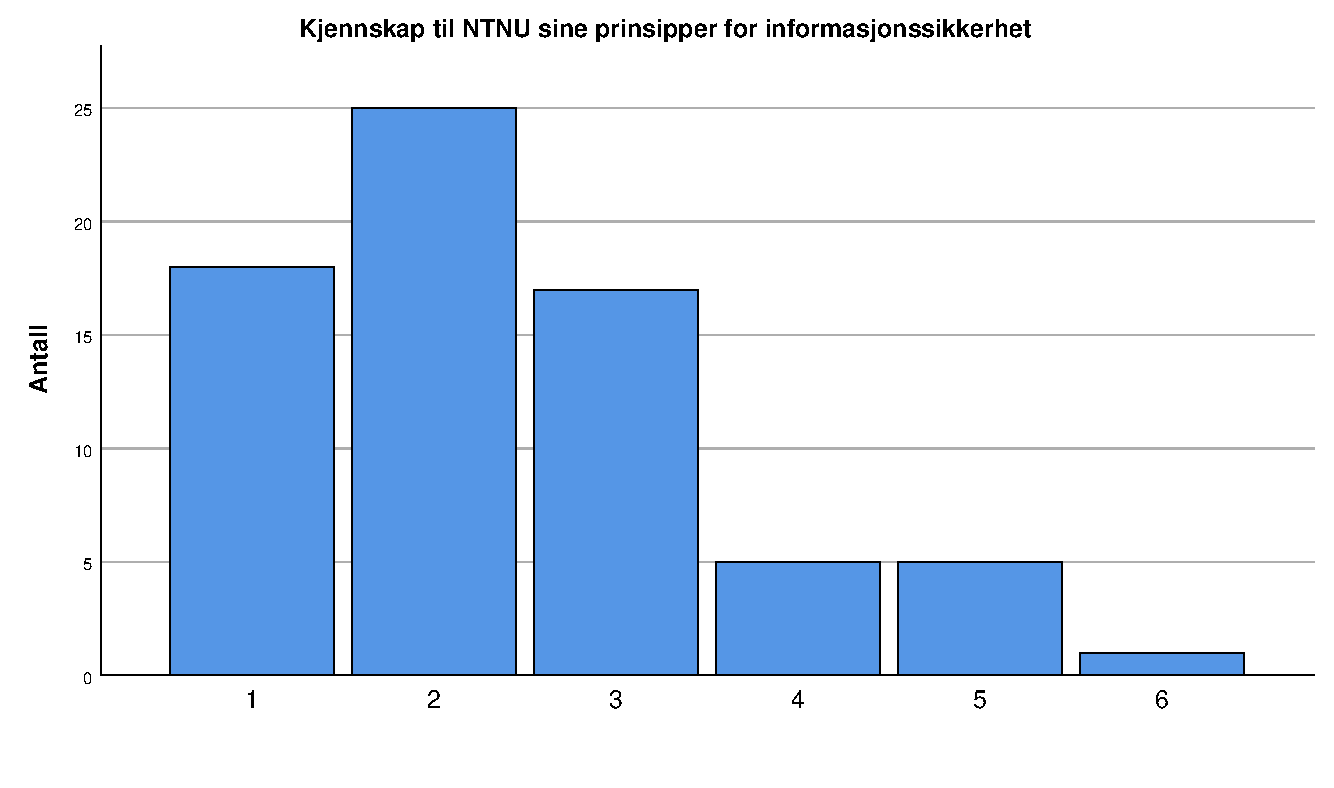
\includegraphics[scale=0.5]{case_2/bilder/spss/InfoSecPolicy.pdf}
    \caption[InfoSecPolicy]{Kjennskap til NTNU sine prinsipper for informasjonssikkerhet}
    \label{fig:InfoSecPolicy}
\end{figure}

Det viser seg at hypotesen vi hadde stemte. Det er lite kjennskap til dokumentasjon på informasjonssikkerhet. Dersom disse dokumentene skal være noe mer enn hyllevarmere må det komme bedre informasjon.


%---------------------------------------Oversikt---------------------------------
\section{Respondentenes egen oversikt}
Her så var vi interessert i å finne ut om når de fant ut at kontoen var blitt kompromittert. Det viser seg at det ikke stemte. Over 60\% av respondentene viste ikke at kontoen var blitt kompromittert før Seksjon for Digital Sikkerhet ringte, og kun 20\% svarte at de fant ut av det før og resten svarte at de ikke vet.
\begin{figure}[H]
    \centering
    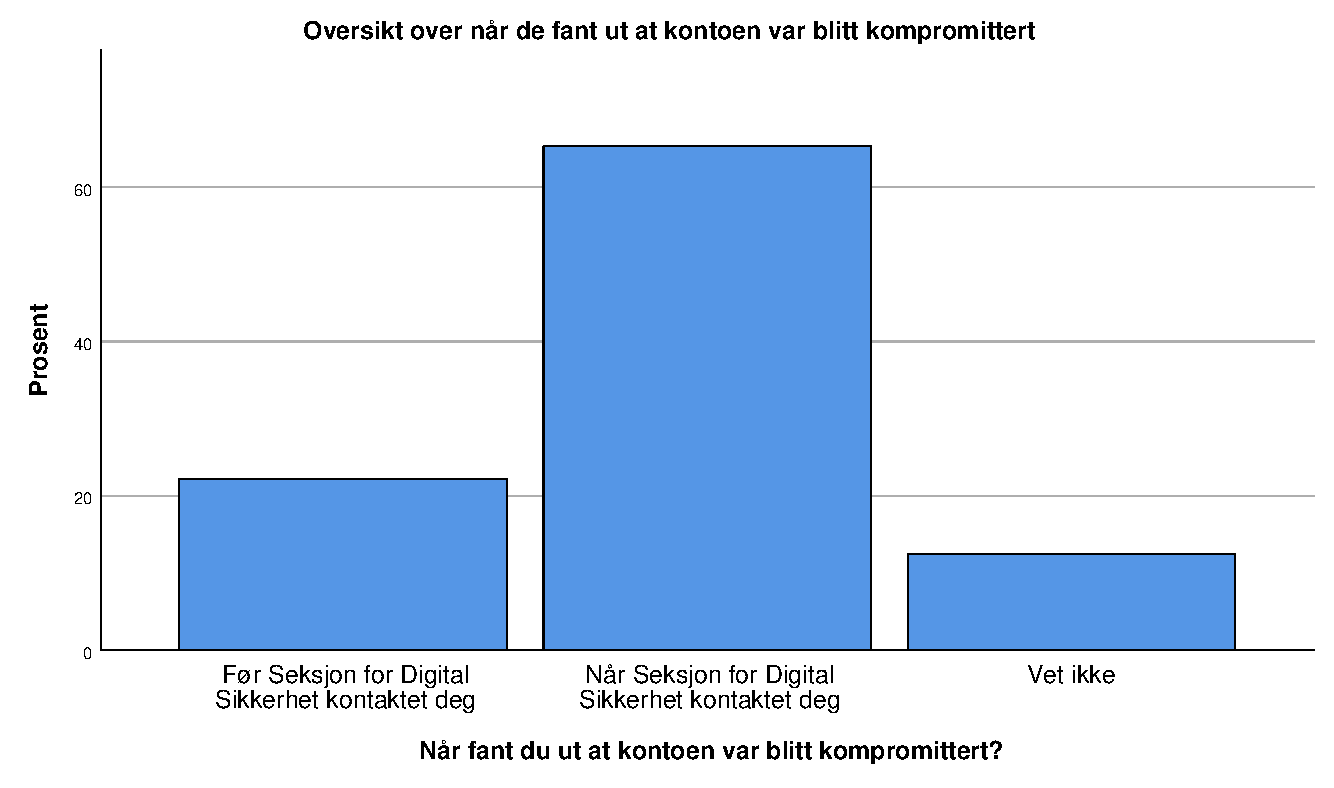
\includegraphics[scale=0.5]{case_2/bilder/spss/Fant_ut_kompromittert.pdf}
    \caption[fant-ut-kompromittert]{Viser når de fant ut at de var blitt kompromittert}
    \label{fig:fant-ut-kompromittert}
\end{figure}
Hypotesen vår her var korrekt. De vet ikke at de har blitt kompromittert før de blir kontaktet.


Respondentene svarte her at kontoen har vært kompromittert mindre enn tre måneder før Seksjon for Digital Sikkerhet ringte. Denne statsistikken kan vi ikke si noe med 100\% sannsynlighet om, fordi halvveis i undersøkelsen fikk vi tilbakemeldiner på at det var flere som ikke vil fullføre spørreundersøkelsen siden dette svaret var obligatorisk. Vi fjernet da kravet om å svare ca halvveis ut i undersøkelsen.  MÅ OMFORMULERES!!!! 
\begin{figure}[H]
    \centering
    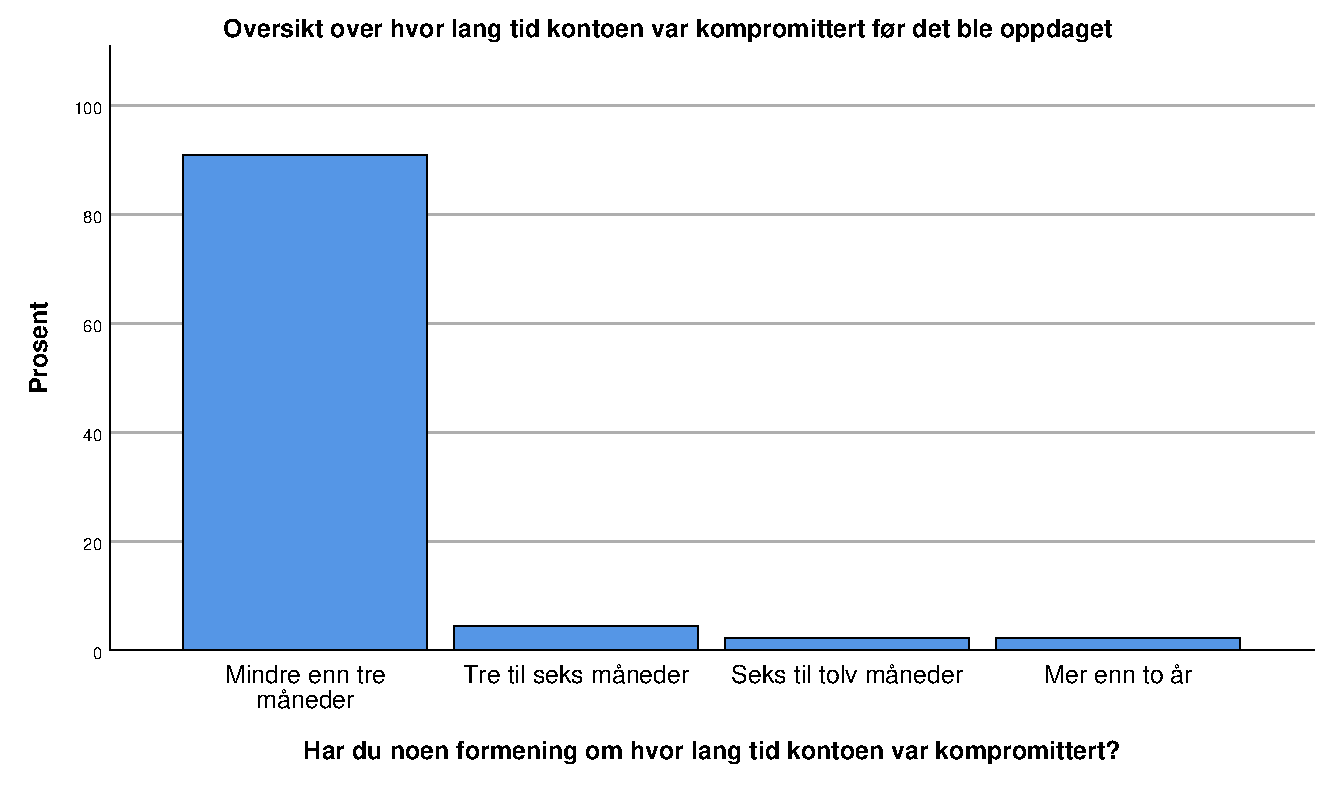
\includegraphics[scale=0.5]{case_2/bilder/spss/lang_tid_konto_kompromittert.pdf}
    \caption[fant-ut-kompromittert]{Viser når de fant ut at de var blitt kompromittert}
    \label{fig:fant-ut-kompromittert}
\end{figure}

\subsection{Formening om hvordan det skjedde}
Dette spørsmålene handlet om respondentene hadde noen formening om hvordan kontoen ble kompromittert. Affinitetsdiagramet viser at respondentene i hovedsak ikke har noen formening om hvordan kontoen ble kompromittert. Over 85\% svarte at de ikke hadde noen formening om hvordan kontoen ble kompromittert. MULIG FOR FEILTOLKING AV SVAR
\begin{figure}[H]
    \centering
    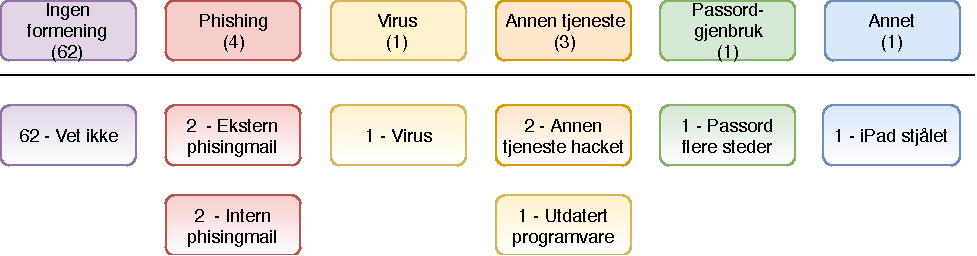
\includegraphics[scale=0.8]{case_2/bilder/Affinitetsdiagram.pdf}
    \caption[affinitetsdiagram]{Affinitetsdiagram av respondentenes formening over hvordan kontoen ble kompromittert}
    \label{fig:case2-affinitetsdiagram}
\end{figure}

\subsection{Konklusjon}
Ut fra svarene kan en konkludere med at de som får kontoen kompromittert i hovedsak ikke vet at den har blitt kompromittert eller når den ble kompromittert. De vet heller stort sett ikke hvordan det har skjedd. 

%---------------------------------------BRUKER- OG PASSORDVANER---------------------------------
\section{Bruker- og passordvaner}

Som vi kan se i figur \ref{fig:epost-jobb} under, bruker over 60\% av respondentene NTNU e-posten til å registrere seg på tjenester i forbindelse med jobb.
\begin{figure}[H]
    \centering
    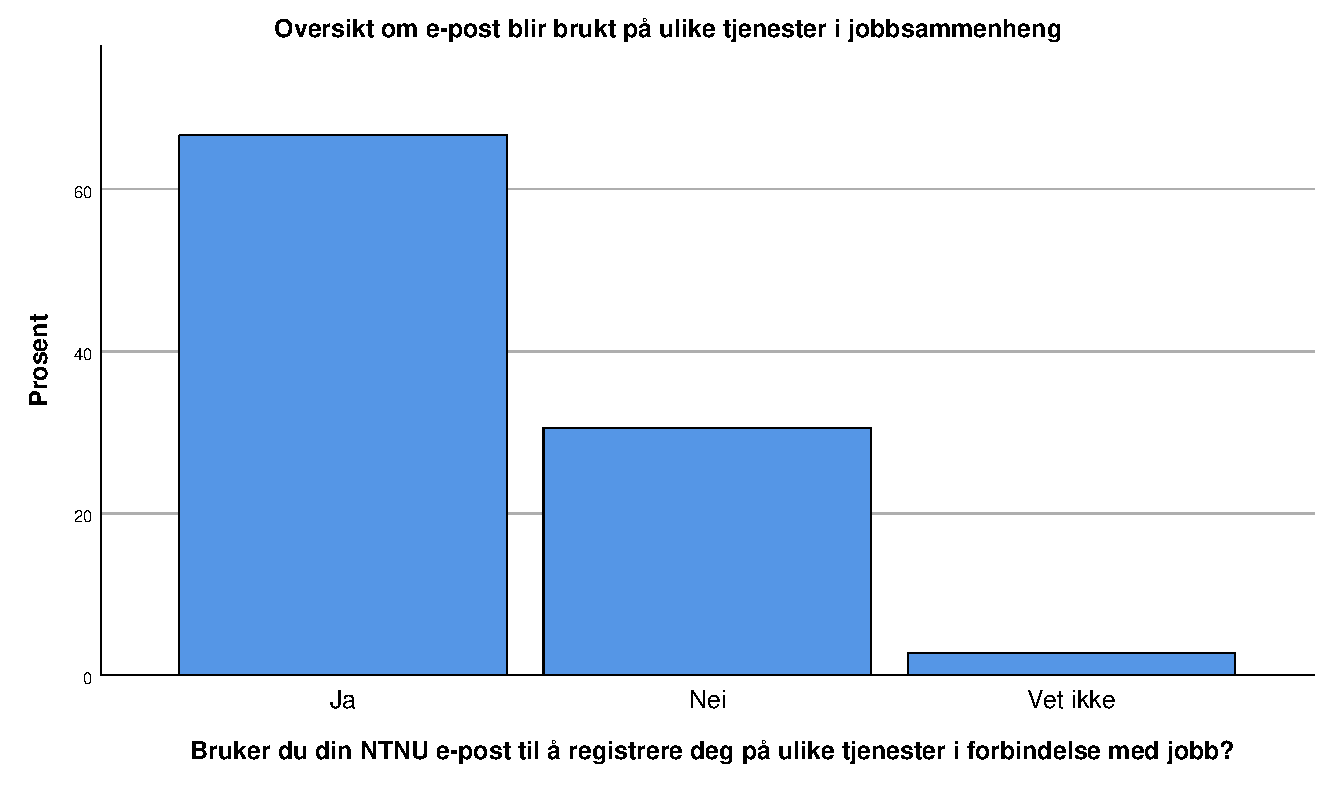
\includegraphics[scale=0.5]{case_2/bilder/spss/epost_jobb.pdf}
    \caption[epost-jobb]{Viser hvor mange som bruker NTNU e-post til andre jobbrelaterte tjenester}
    \label{fig:epost-jobb}
\end{figure}
Hypotesen vår stemte. Over halvparten bruker NTNU e-posten til å registrere seg på tjenester i forbindelse med jobb. 

48,6\% av respondentene bruker NTNU e-posten sin til private tjenester. Den samme andelen gjør ikke det og de restende (2,8\%) har svart at de ikke vet. Dette blir vist i figur \ref{fig:epost-privat}.
\begin{figure}[H]
    \centering
    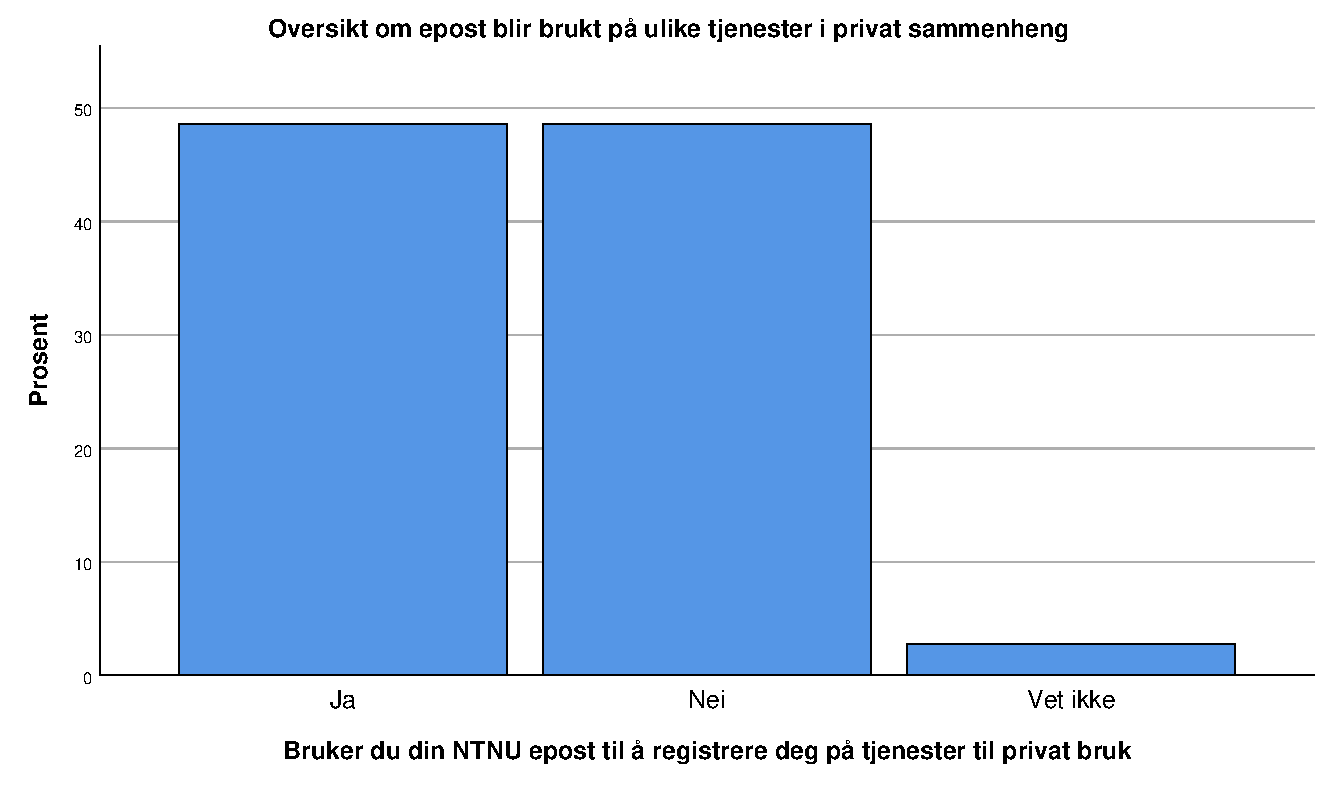
\includegraphics[scale=0.5]{case_2/bilder/spss/epost_privat.pdf}
    \caption[epost-privat]{Viser hvor mange som bruker NTNU e-post til private tjenester}
    \label{fig:epost-privat}
\end{figure}
Hypotesen vår var korrekt, under halvparten bruker NTNU e-posten sin til private tjenester. 

Over 50\% av respondentene bruker NTNU passordet på flere tjenester. Dette vises i figuren under. 
\begin{figure}[H]
    \centering
    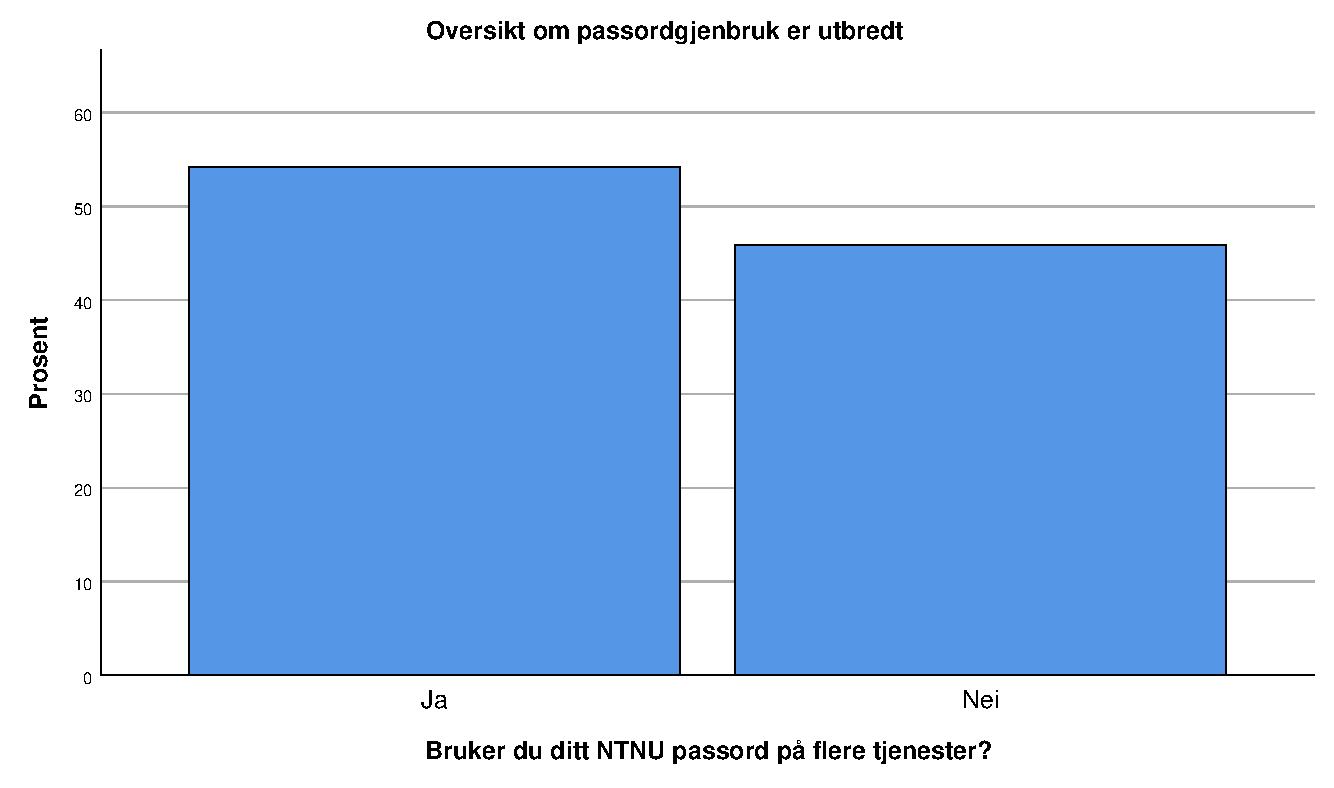
\includegraphics[scale=0.5]{case_2/bilder/spss/passordgjenbruk.pdf}
    \caption[passordgjenbruk]{Oversikt over gjenbruk av NTNU passord}
    \label{fig:passordgjenbruk}
\end{figure}
Hypotesen vår var her korrekt, passordgjenbruk er utbredt på NTNU. 

Over 80\% av respondentene svarte at de ikke brukte regler til å generere passord. Det er mulig for feiltolkning av spørsmålet, i og med at regler kan bety to forskjellige ting. Det kan bety regle, i form av ``Lisa-gikk-til-NTNU'' for NTNU-passord, eller så kan man tolke det som en regel. 
\begin{figure}[H]
    \centering
    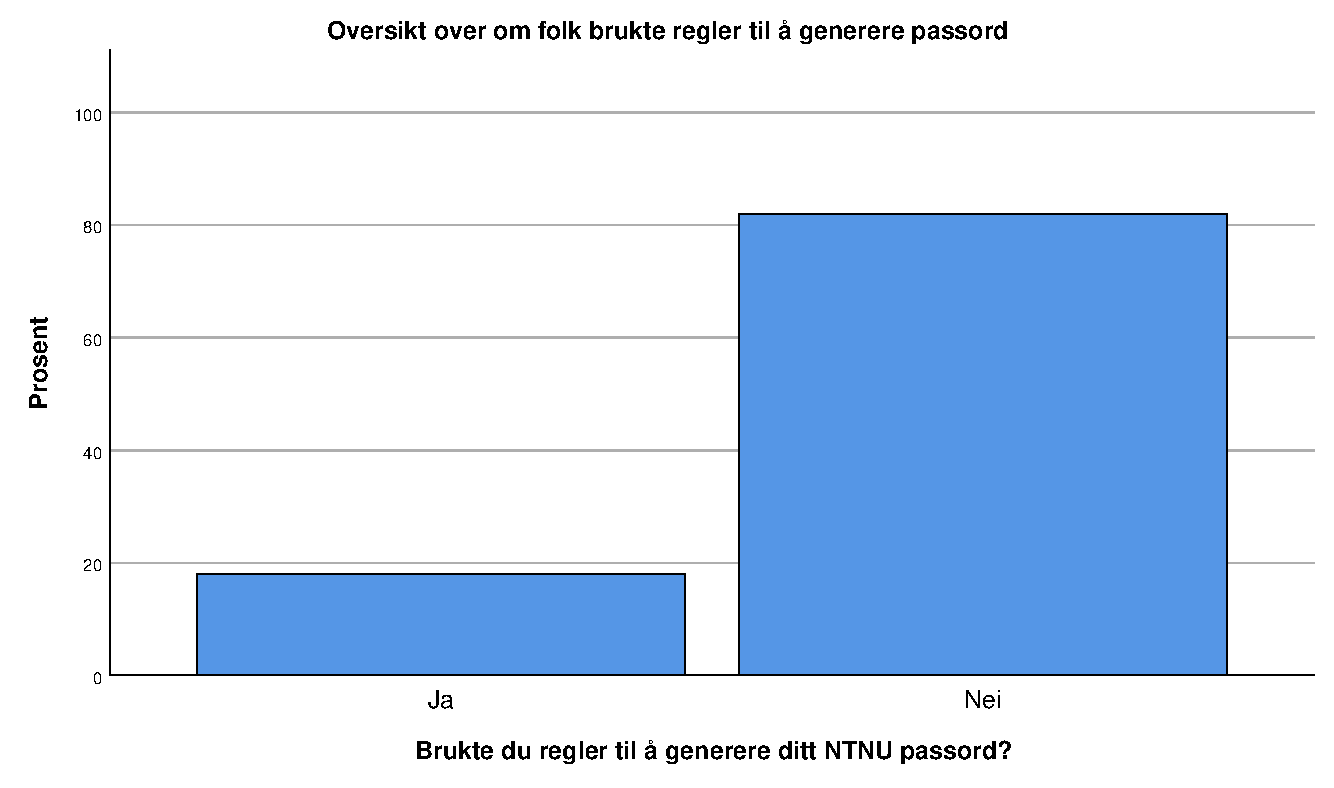
\includegraphics[scale=0.5]{case_2/bilder/spss/regler_passord.pdf}
    \caption[passordregler]{Viser hvor mange som bruker passordregler}
    \label{fig:passordregler}
\end{figure}
Vi kan derfor ikke si om hypotesen vår ble bekreftet eller avkreftet.

Over 80\% av respondentene har passord som er mellom 8-11 tegn. Resterende fordelte seg likt utover de andre valgene. 
\begin{figure}[H]
    \centering
    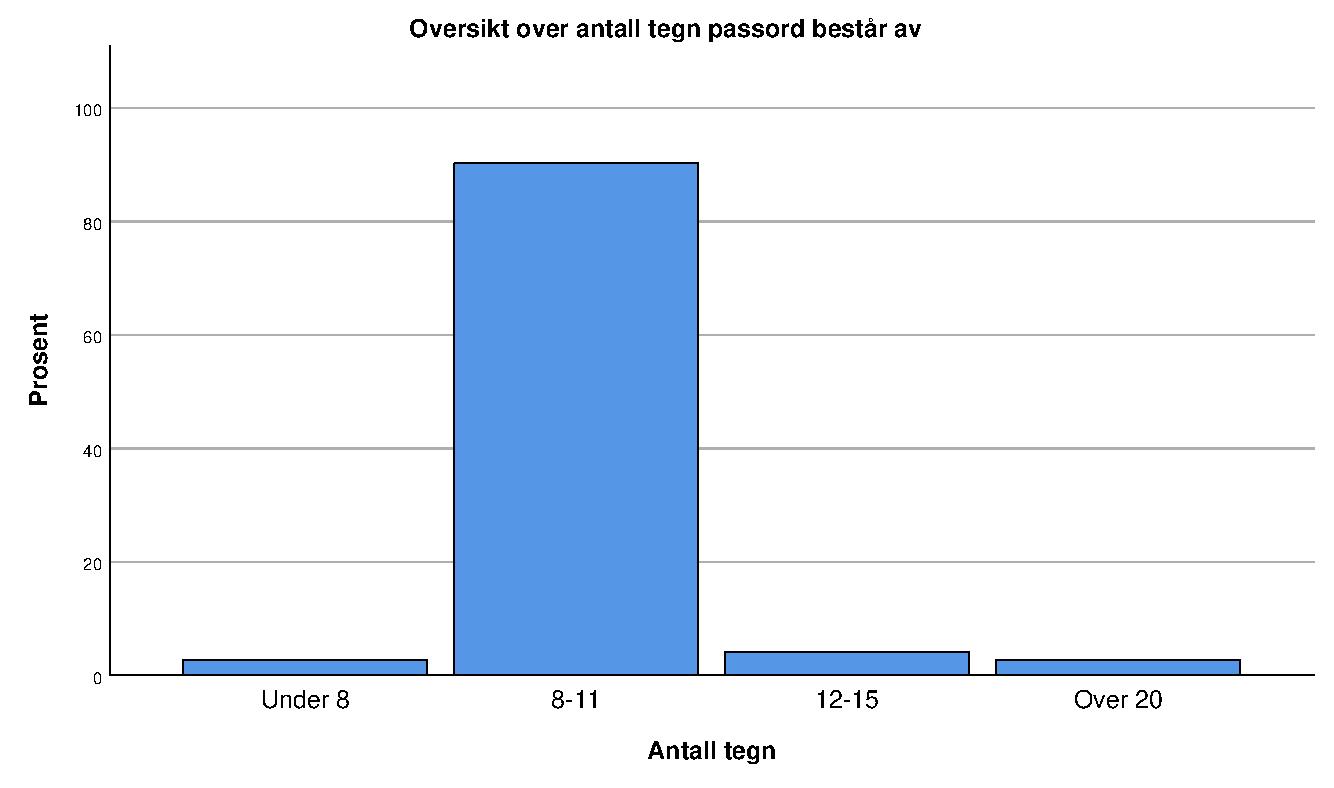
\includegraphics[scale=0.5]{case_2/bilder/spss/antall_tegn.pdf}
    \caption[antalltegn]{Antall tegn på passord}
    \label{fig:antalltegn}
\end{figure}
Hypotesen vår var korrekt, de fleste bruker passord som er under 12 tegn. Burde splitte opp 8-11!!!

Figur \ref{fig:bytter-passord} viser statistikken over hvor ofte respondentene bytter passord. Over 50\% sier at de bytter passord sjeldnere enn hvert andre år, over 20\% sier at de bytter hvert andre år, rett under 20\% sier at de bytter hvert år og resten sier at de bytter hver sjette måned. 
\begin{figure}[H]
    \centering
    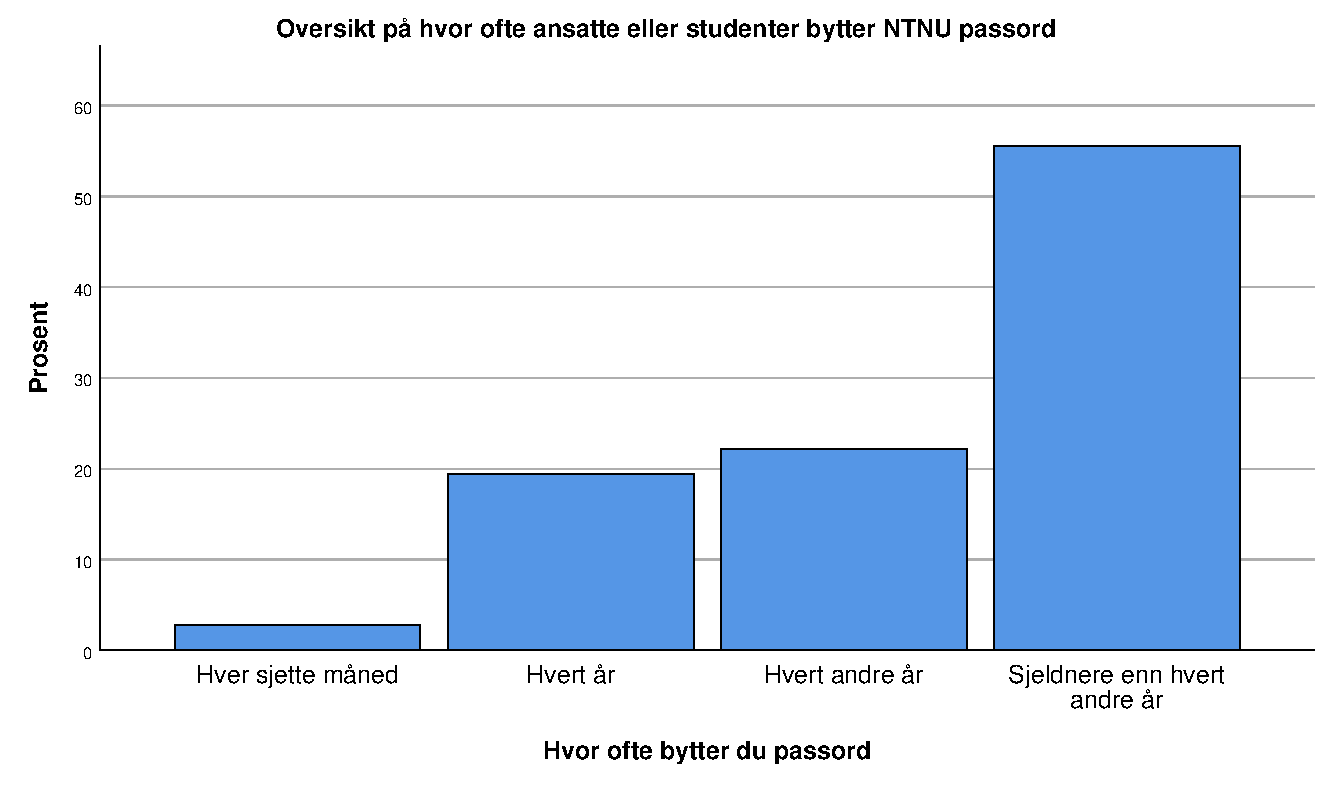
\includegraphics[scale=0.5]{case_2/bilder/spss/bytter_passord.pdf}
    \caption[bytter-passord]{Viser hvor ofte de bytter passord}
    \label{fig:bytter-passord}
\end{figure}
Hypotesen var korrekt, flertallet av respondentene bytter passord sjeldnere enn hvert andre år. I henhold til IT-reglementet over passord, brukernavn og authentiseringsdata så skal passord byttes hver sjette måned og tvungen passordbytte hvert år. Dette viser at respondentene ikke kjent med IT-reglementet og reglementet blir ikke overholdt.

Her så ser vi antallet som sier at de har fått opplæring i passordsikkerhet fra NTNU. Ut fra tabellen ser vi at under 80\% av respondentene sier at de ikke har fått opplæring i passordsikkerhet. 15\% sier at de ikke vet om de har fått opplæring og resten sier at de har fått det. Figur \ref{fig:passordsikkerhet} viser dette. 
\begin{figure}[H]
    \centering
    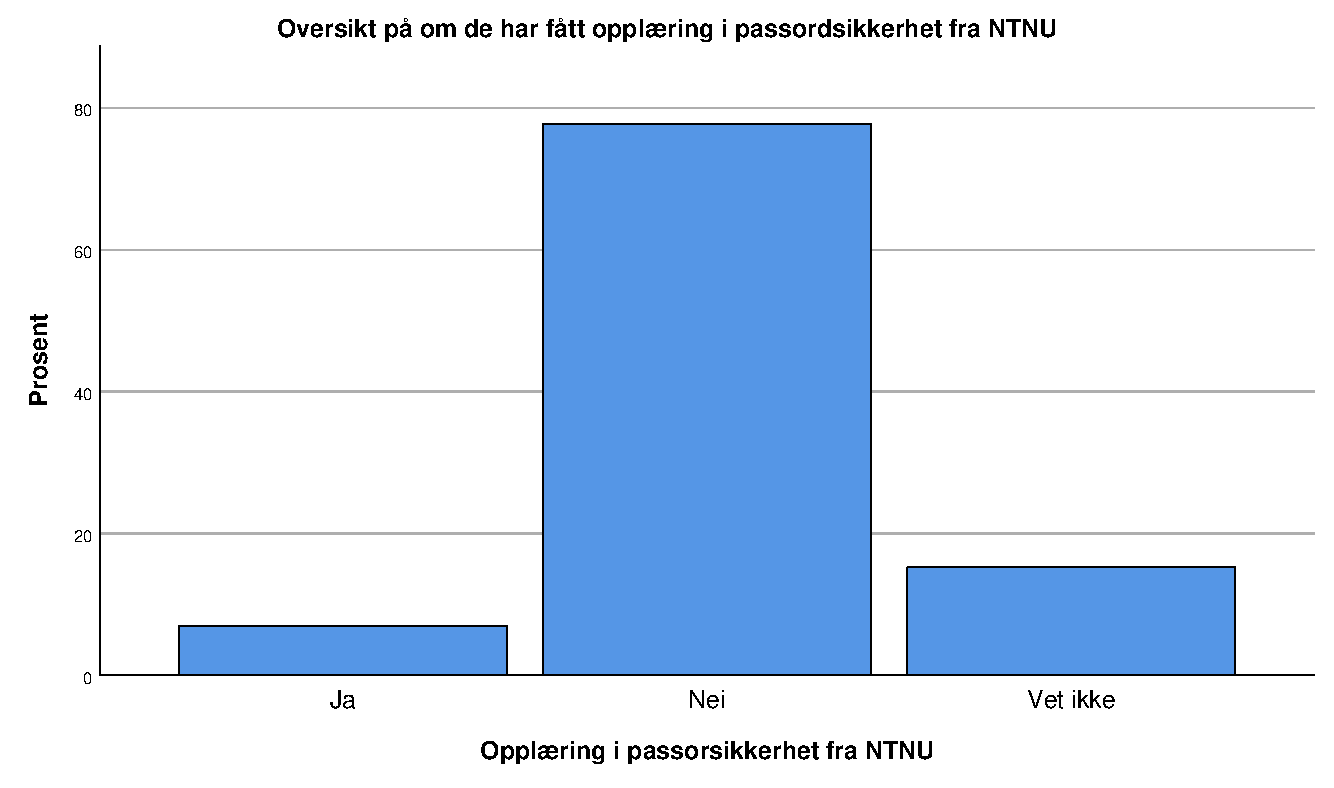
\includegraphics[scale=0.5]{case_2/bilder/spss/opplaring_passordsikk_NTNU.pdf}
    \caption[passordsikkerhet]{Viser hvor mange som har fått opplæring i passordsikkerhet}
    \label{fig:passordsikkerhet}
\end{figure}
Vår hypotese her stemte, de ansatte har ikke fått tilstrekkelig opplæring i passordsikkerhet.  


\subsection{Konklusjon}
Ut fra spørsmålene om bruker- og passordvaner kan vi konkludere med at passordsikkerheten til de kompromitterte er lav. De fleste har brukt sitt NTNU passord på flere tjenester og over halvparten har også brukt sin NTNU e-post på andre tjenester. Dette er mest utbredt på tjenester relatert til jobben. I tillegg til det benytter mange seg av passord som er mellom 8-11 tegn, noe som er rett over minimumsgrensen. De fleste bytter passord sjeldnere enn hvert andre år, selv om retningslinjer for behandling av brukernavn, passord og andre autentiseringsdata \cite{RetnBPA} anbefaler å bytte det hver tolvte måned. 

Noe av årsaken til dette denne lave kompetanse kan være at de ikke har fått tilstrekkelig innføring i passordsikkerhet fra NTNU og IT-reglementet som er krav til at de skal lese igjennom sier lite om bruker- og passordvaner. IT-reglementet sier ingenting om antall tegn på passord eller hvor ofte passordet skal byttes, dette står som en anbefaling fra orakeltjenesten om hva du skal forholde deg til når du lager passord og hvor ofte du skal bytte.   

%----------------------------------------PHISHING---------------------------------
\section{Phishing}
Over 70\% av respondentene sa at de har oppdaget phishing e-post en eller flere ganger på sin NTNU e-post, og rett under 20\% som ikke har oppdaget phishing e-post. Resten av respondentene svarte at de ikke vet. Dette vises i diagrammet under \ref{fig:oppdaget-phishing}.
\begin{figure}[H]
    \centering
    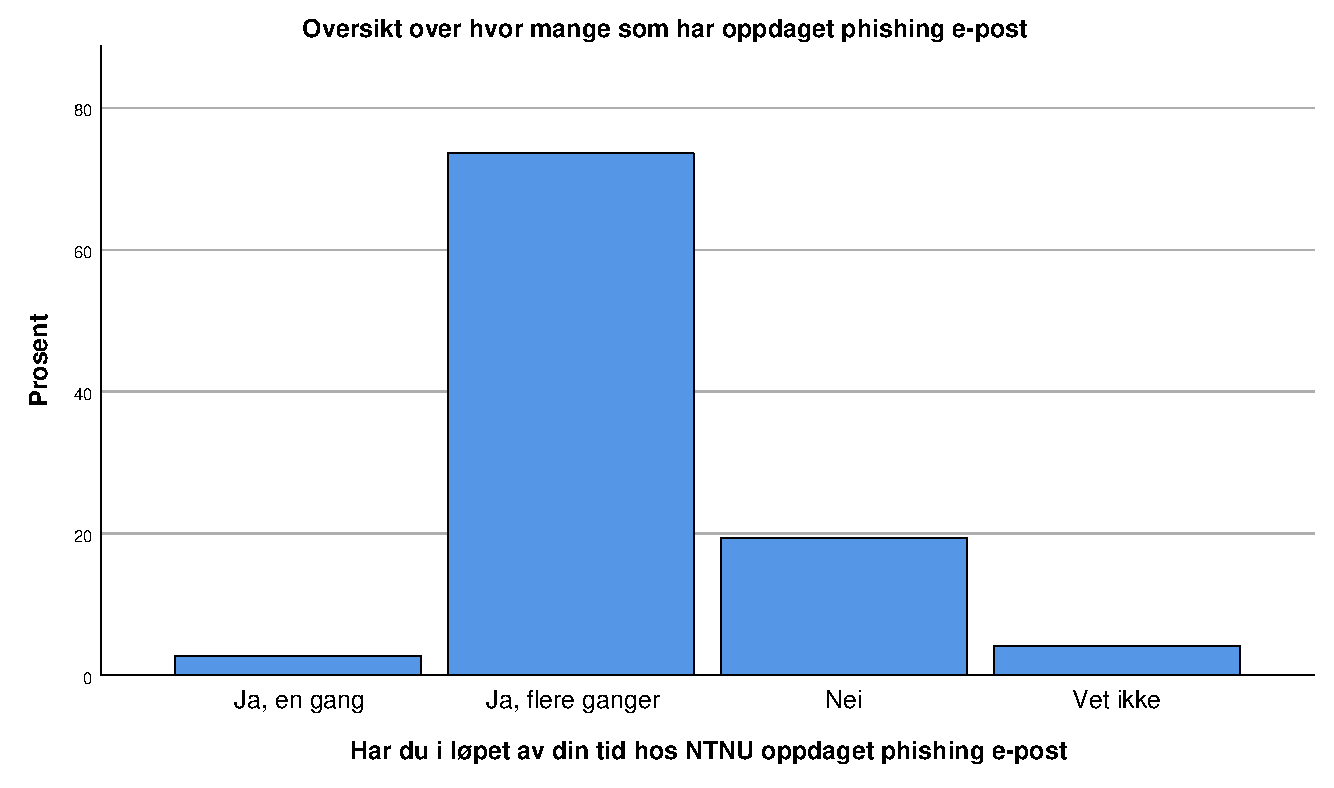
\includegraphics[scale=0.5]{case_2/bilder/spss/oppdaget_phish.pdf}
    \caption[oppdaget-phishing]{Viser hvor mange som har oppdaget phishing e-post}
    \label{fig:oppdaget-phishing}
\end{figure}
Hypotesen vår er sann. Phishing er en svært utbredt angrepsvektor. 

Over 70\% av respondentene sier at de ikke har blitt lurt av phishing e-post, og under 20\% sier at de har blitt lurt. Som vist i tabellen under \ref{fig:lurt-av-phishing}. 
\begin{figure}[H]
    \centering
    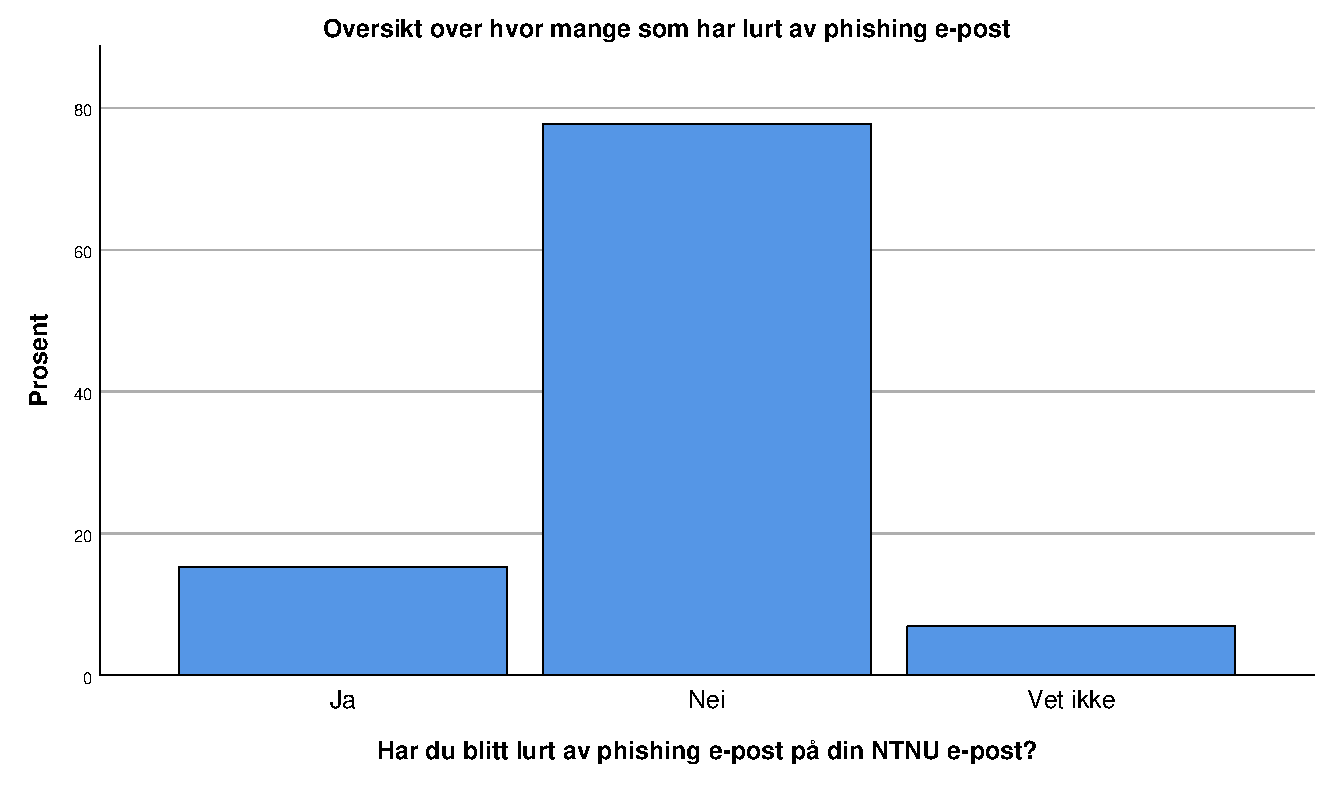
\includegraphics[scale=0.5]{case_2/bilder/spss/lurt_phish.pdf}
    \caption[lurt-av-phishing]{Viser hvor mange som sier de har blitt lurt av phishing}
    \label{fig:lurt-av-phishing}
\end{figure}
Ut fra dataen, kan vi si at vår hypotese ikke stemte.   

\subsection{Konklusjon}


%----------------------------------------STATISTISK ANALYSE---------------------------------
\section{Statistisk analyse}
I denne delen bruker vi statistiske analyseverktøy for å finne relasjoner. De analysene vi fremhever her er de vi anså som mest relevante. De mindre relevante er plassert i vedlegg \ref{vedlegg:statanalys}, og de som enten ble ansett som urelevante eller som hadde lite signifikans har blitt utelatt. Som en generell regel for utføring av analysen har vi valgt et signifikansnivå på: \[\alpha \leq 0,05\]

\subsection{ANOVA på alder mot bevissthet og kjennskap}
Denne testen sjekker om det er signifikans mellom alder på respondenten, og hvor bevisste de er på sikkerhet og hvor godt de kjenner til de ulike retningslinjene og reglementene. Alle spørsmålene er besvart på en skala fra 1 til 6, der 1 er lite bevisst eller kjent, og 6 er svært bevisst eller kjent. I tabellen under beskrives svarene til datasettet som er analysert. 
\begin{figure}[H]
    \centering
    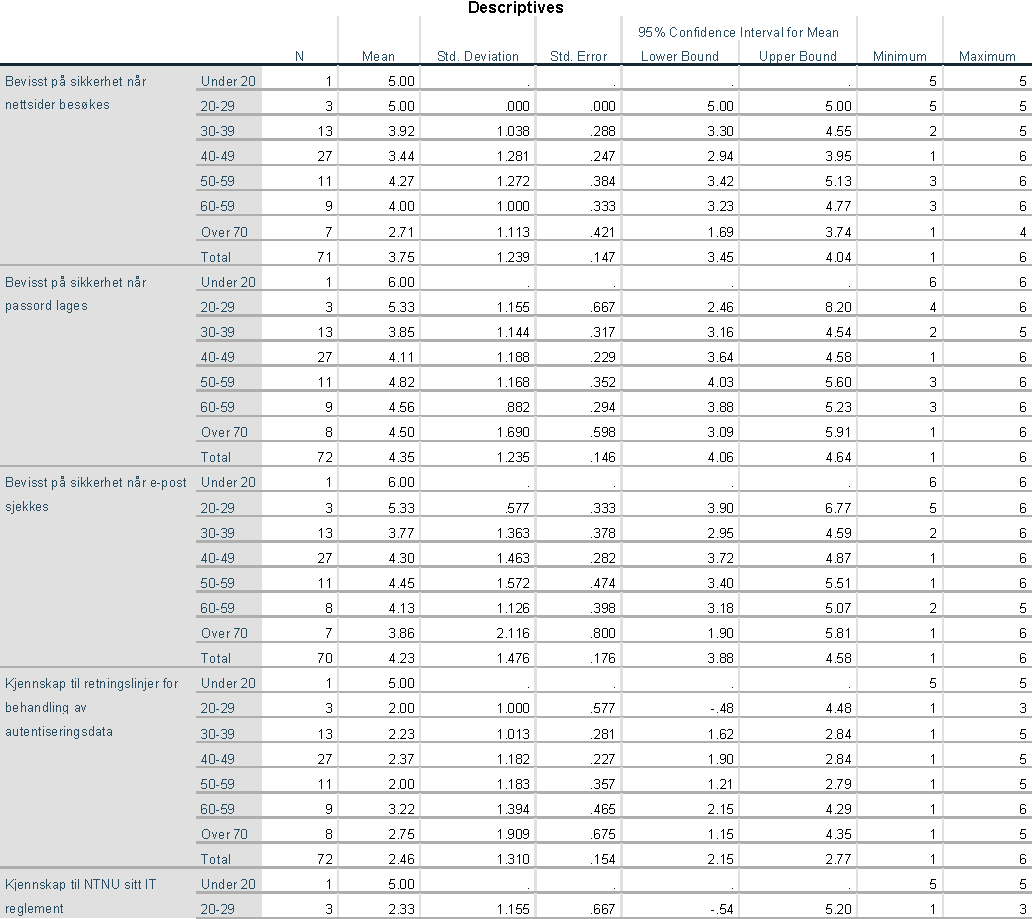
\includegraphics[scale=0.7]{case_2/bilder/spss/anova_ttest/alder_bevissthetogkjennskap_descriptive_1.pdf}
    \caption[alder-bevissthetogkjennskap-descriptive-1]{Descriptive av alder mot bevissthet på sikkerhet og kjennskap til retningslinjer, del 1}
    \label{fig:alder-bevissthetogkjennskap-descriptive-1}
\end{figure}

\begin{figure}[H]
    \centering
    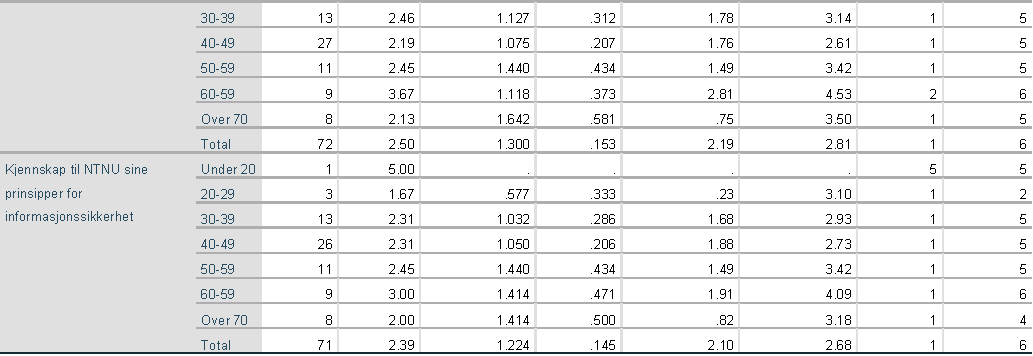
\includegraphics[scale=0.7]{case_2/bilder/spss/anova_ttest/alder_bevissthetogkjennskap_descriptive_2.pdf}
    \caption[alder-bevissthetogkjennskap-descriptive-2]{Descriptive av alder mot bevissthet på sikkerhet og kjennskap til retningslinjer, del 2}
    \label{fig:alder-bevissthetogkjennskap-descriptive-2}
\end{figure}


\begin{figure}[H]
    \centering
    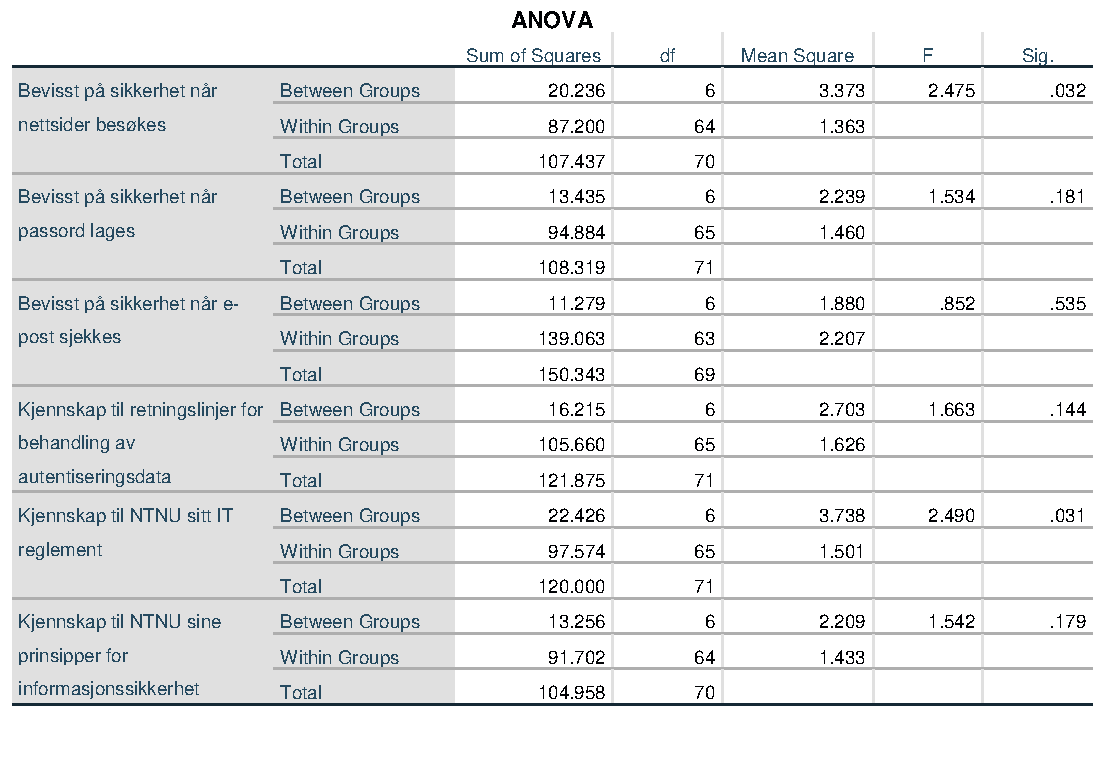
\includegraphics[scale=0.7]{case_2/bilder/spss/anova_ttest/alder_bevissthetogkjennskap_anova.pdf}
    \caption[alder-bevissthetogkjennskap-ANOVA]{ANOVA av alder mot bevissthet på sikkerhet og kjennskap til retningslinjer}
    \label{fig:alder-bevissthetogkjennskap-ANOVA}
\end{figure}

En post-hoc test kunne ikke kjøres her fordi en av kategoriene bare hadde ett svar. 

\subsection{ANOVA på år ved NTNU mot passord-, e-post- og andre brukervaner}
Denne testen sjekker om det er signifikans mellom antall år respondenten har vært hos NTNU, og om de bruker NTNU e-posten sin på andre tjenester, om de har blitt lurt av phishing og om de benytter sitt NTNU passord på flere tjenester. I tabellen under beskrives svarene til datasettet vi skal analysere.
\begin{figure}[H]
    \centering
    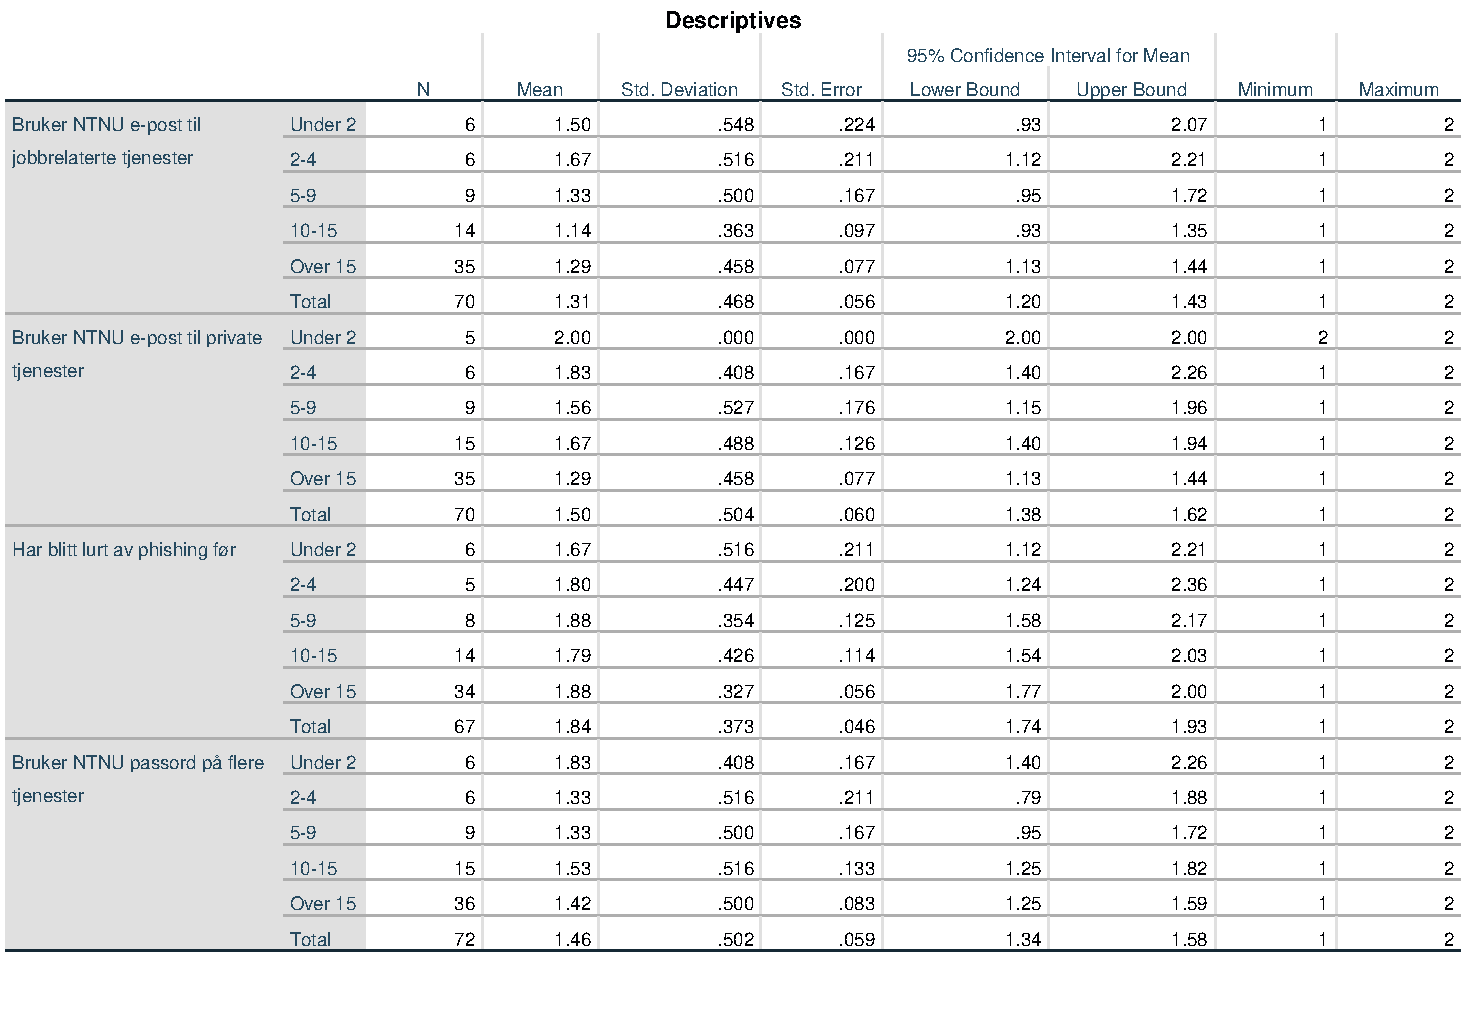
\includegraphics[scale=0.5]{case_2/bilder/spss/anova_ttest/ansiennitet_diverse_descriptive.pdf}
    \caption[ansiennitet-diverse-descriptive]{Descriptive av år ved NTNU mot passord-, e-post- og andre brukervaner}
    \label{fig:ansiennitet-diverse-descriptive}
\end{figure}

\begin{figure}[H]
    \centering
    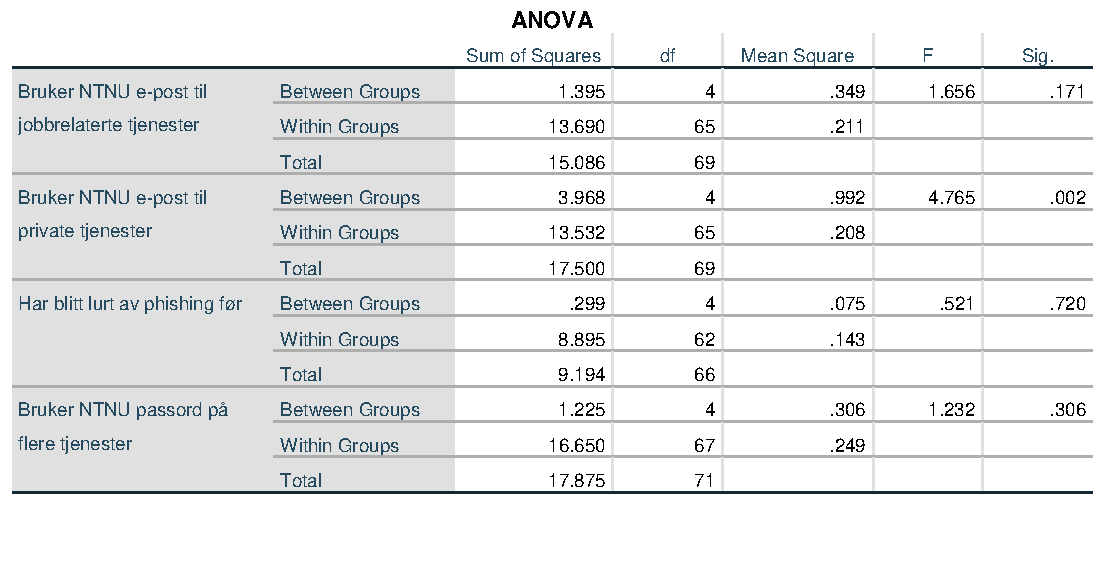
\includegraphics[scale=0.7]{case_2/bilder/spss/anova_ttest/ansiennitet_diverse_anova.pdf}
    \caption[ansiennitet-diverse-ANOVA]{ANOVA av år ved NTNU mot passord-, e-post- og andre brukervaner}
    \label{fig:ansiennitet-diverse-ANOVA}
\end{figure}

Siden det er signifikans på de som bruker NTNU e-post til private tjenester (\(\alpha \leq 0,05\)), ble en post-hoc test kjørt for å se om det var noen ytterligere signifikans mellom gruppene. Grunnet plassbesparelse er bare de variablene som inkluderte signifikans tatt med i rapporten. 
\begin{figure}[H]
    \centering
    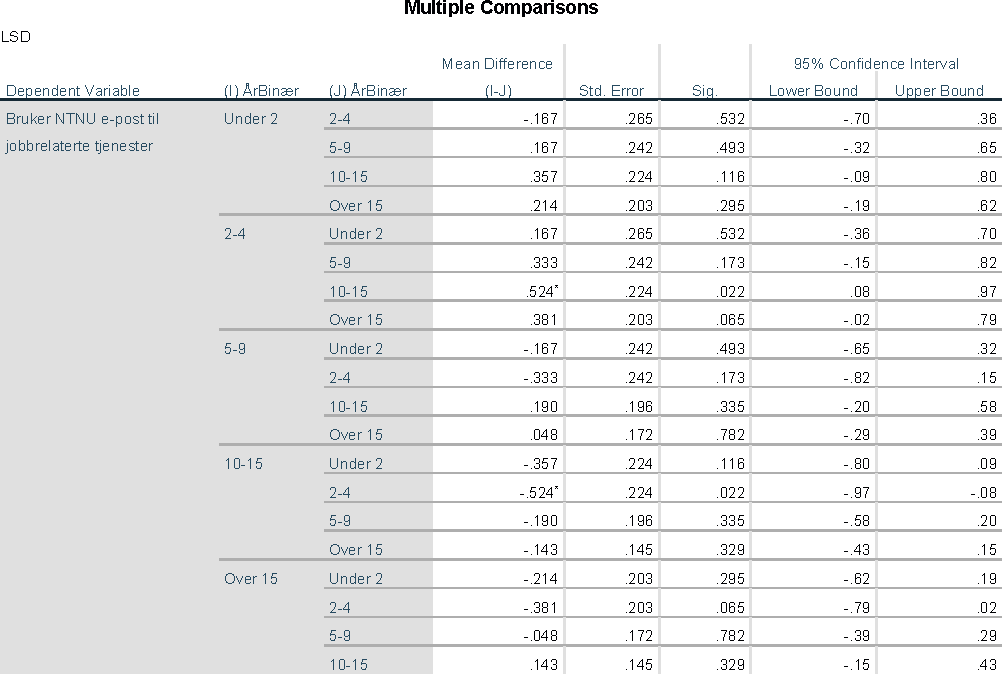
\includegraphics[scale=0.7]{case_2/bilder/spss/anova_ttest/ansiennitet_diverse_posthoc_1.pdf}
    \caption[ansiennitet-diverse-posthoc-1]{Post-hoc av år ved NTNU mot passord-, e-post- og andre brukervaner, del 1}
    \label{fig:alder-bevissthetogkjennskap-descriptive-1}
\end{figure}

\begin{figure}[H]
    \centering
    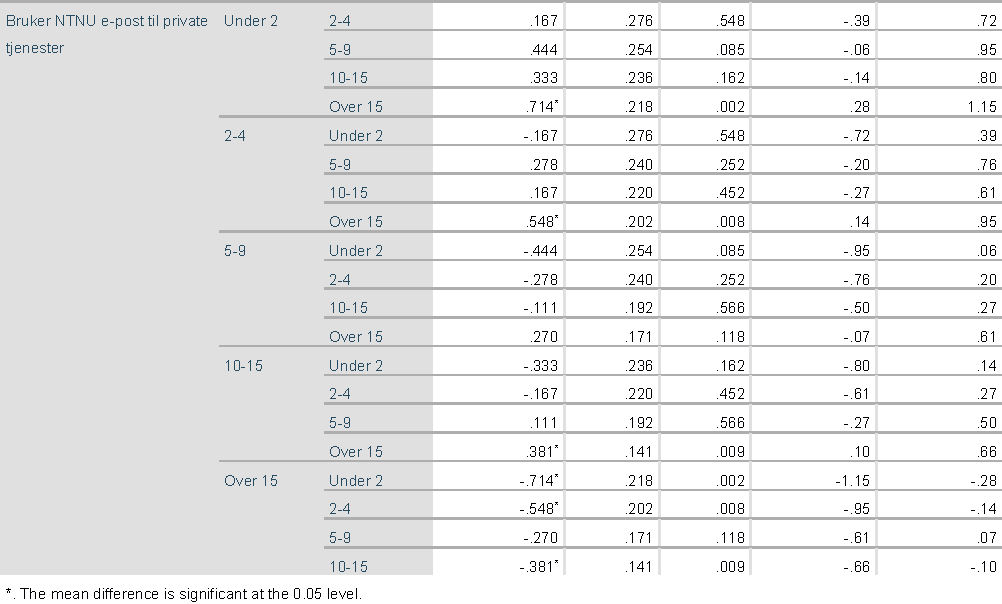
\includegraphics[scale=0.7]{case_2/bilder/spss/anova_ttest/ansiennitet_diverse_posthoc_2.pdf}
    \caption[ansiennitet-diverse-posthoc-2]{Post-hoc av år ved NTNU mot passord-, e-post- og andre brukervaner, del 2}
    \label{fig:alder-bevissthetogkjennskap-descriptive-2}
\end{figure}

\subsection{ANOVA på alder mot passord-, e-post- og andre brukervaner}
Siden det ble funnet signifikans på antall år ved NTNU og bruk av NTNU e-post på private tjenester, kunne det være sannsynlig at dette også korrelerte med alder. Det er logisk å tro at jo lenger tid en har tilbringet ved NTNU, jo eldre er personen. Derfor ble det kjørt en korrelasjonstest på alder og antall år ved NTNU for å teste dette. I tabellen under kan vi se at det er en sterk positiv korrelasjon (\(\alpha \le 0,01\)) mellom alder og tid ved NTNU.

\begin{figure}[H]
    \centering
    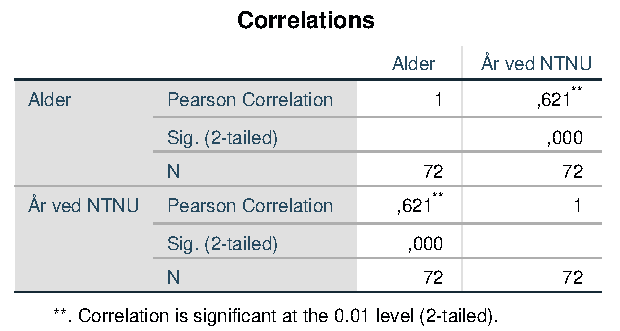
\includegraphics[scale=1]{case_2/bilder/spss/anova_ttest/alder_aarvedNTNU_korrelasjon.pdf}
    \caption[alder-aarvedNTNU-korrelasjon]{Korrelasjon mellom alder og antall år ved NTNU}
    \label{fig:alder-aarvedNTNU-korrelasjon}
\end{figure}

Basert på resultatene er det grunnlag for å tro at siden jo eldre respondenten som har fått sin konto kompromittert er, jo mer sannsynlig er det at personen har benyttet e-posten på private tjenester, basert på resultatene i figur \ref{fig:ansiennitet-diverse-ANOVA} i forrige seksjon.

\subsection{ANOVA på år ved NTNU mot bevissthet og kjennskap}
Det ble ikke funnet noen signifikans mellom gruppene. Det er ingen grunn til å tro at tid ved NTNU har noe til felles med hvor bevisst du er på sikkerhet, eller hvor godt kjent du er med de styrende og rutinemessige dokumentene. Se vedlegg \ref{aarvedNTNU-mot-bevissthetogkjennskap} for ANOVA analysen.


\subsection{Independent sample t-test på kjønn mot bevissthet og kjennskap}
Det ble ikke funnet noen signifikans mellom gruppene. Vi kan dermed ikke si at det er noen forskjell mellom kjønnene av de som har blitt kompromittert, når det kommer til bevissthet på sikkerhet og kjennskap til retningslinjer. Se vedlegg \ref{kjonn-mot-bevissthetogkjennskap} for Independent Sample t-testen. 



\section{Konklusjon av verktøy}


\subsection{Histogram}


\subsection{Sektordiagram}


\subsection{Affinitetsdiagram}


\subsection{Statistiske analyseverktøy}

\chapter{Rotårsaksidentifisering}
Arbeidet i denne fasen går ut på å identifisere rotårsaken. I foregående fasen ble en rekke mulige årsaker identifisert og analysert, men nå er det tid for å finne den faktiske rotårsaken. Det er mange forskjellige verktøy som kan brukes i denne fasen, men vi har brukt et årsak-virkningsdiagram for vårt utgangspunkt.

\section{Årsak-virkningsdiagram}
Et årsak-virkning diagram er et diagram som analyserer forholdene mellom et problem og dets årsaker. Det kombinerer aspekter ved idémyldring med systematisk analyse. Det finnes to typer årsak-virkning diagrammer, fiskebeindiagram og prosessdiagram. Mens et prosessdiagram er mer direkte fokusert på problemet på innsiden av forretningsprosessene, er et fiskebeindiagram en mer generell tilnærming for å adressere alle potensielle årsaker\cite{RCA}. I dette caset har vi valgt et fiskebeindiagram på bakgrunn av at årsakene er spredt over flere variabler. 

\subsection{Ønsket utbytte}
Ved bruk av dette verktøyet ønsker vi å sitte igjen med en visuell fremstilling av rotårsakene til problemet. Dette vil gjøres ved å identifisere hva som skaper årsakene vi har funnet fram til i foregående fase. 

\subsection{Gjennomføring}
Det er anbefalt å bruke en tusjtavle for å tegne opp fiskebeindiagrammet, men vi valgte å bruke det nettbaserte programmet draw.io \cite{drawio}. Draw.io er laget for å skape diagrammer med flere brukere involvert i sanntid. De hadde en egen mal for fiskebeindiagram som vi valgte å gå ut fra. Stegene vi fulgte i prosessen er hentet fra boka om rotårsaksanalyse \cite{RCA} og ble som følger:

\begin{enumerate}
    \item Først ble problemet definert og skrevet i slutten av fiskebeindiagrammet.
    \item Deretter ble hovedkategoriene skrevet ned i bokser. Disse er direkte tilknyttet resultatene fra analysen.
    \item Videre startet vi å idémyldre alle mulige årsaker under hver kategori, en kategori om gangen. Disse ble fortløpende skrevet inn i diagrammet.
    \item Til slutt analyserte vi de identifiserte årsakene og bestemte de mest sannsynlige rotårsakene
\end{enumerate}

\subsection{Resultat}
Innledningsvis ble problemet beskrevet som rotårsaken til kompromitterte kontoer ved NTNU. Hovedkategoriene som ble undersøkt for å finne svar på dette, var gjenbruk av innloggingskredentialier tilhørende NTNU, IT-reglementet og andre styringsdokumenter, passordvaner, phishing og oversikt. Både hovedkategoriene og årsakene under disse er i hovedsak basert på dataanalysen, mens noe er basert på kreativ idémyldring. 

\begin{figure}[H]
    \centering
    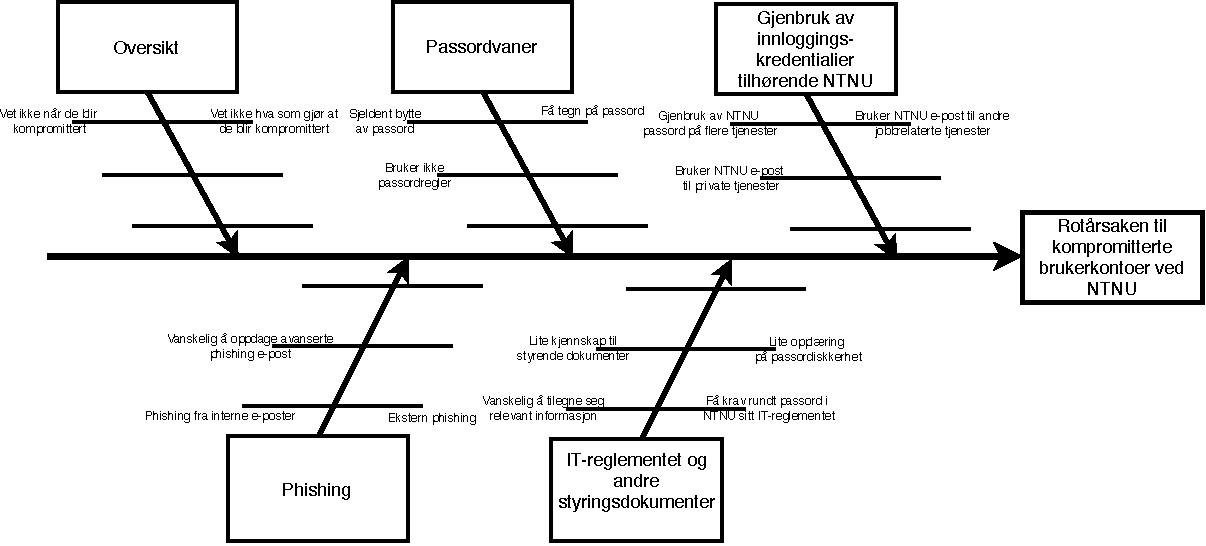
\includegraphics[scale=1.1, angle=90]{case_2/bilder/fiskebein.pdf}
    \label{fig:fiskebein-case2}
    \caption[Fiskebein-case2]{Fiskebeindiagram over hovedkategorier og årsaker}
\end{figure}

Vi har kommet frem til at rotårsaken til kompromitterte kontoer er sammensatt av flere faktorer. Et passord på mellom åtte til elleve tegn i seg selv er ikke nok for at kontoen skal bli kompromittert, men sammen med at de bytter sjeldnere enn hvert andre år gjør at dette blir et problem. I tillegg til dette bruker flertallet NTNU e-posten til andre tjenester, enten til jobbrelatert eller til privat bruk. De bruker også samme NTNU passord på flere tjenester. Dette er noe en burde unngå til en hver tid, og er noe av det vi anser å være blant det mest kritiske. 

Respondentene hadde også liten kjennskap til IT-reglementet og andre styringsdokumenter. De svarte også at de har fått lite opplæring på passordsikkerhet. Vi har lest igjennom IT-reglementet og andre styringsdokumenter, og har kommet frem til at IT-reglementet har for få krav til passord, det var vanskelig å tilegne seg all informasjon på de forskjellige styringsdokumentene da IT-reglementet ikke henviste til noen av retningslinjene. I Retningslinjer for behandling av brukernavn, passord og andre autentiseringsdata \cite{RetnBPA} står det at passordet skal byttes hver 12 måned. Denne retningslinjen er ikke nevnt i IT-reglementet at du skal gjøre deg bekjent med. 

Sammenlagt så viste det oss at respondentene hadde dårlige passordvaner, gjenbruk av innloggingskredentialier tilhørende NTNU og lite kunnskap til IT-reglementet og andre styrende dokumenter. Phishing er også en relevant årsak til kompromitterte kontoer. Phishing e-poster har blitt såpass sofistikerte at det er vanskelig å skille mellom falske og legimite e-poster. \cite{SophPhish}. Rotårsakene er derfor som følger: 

\begin{itemize}
    \item Mistet kontodetaljer av phishing
    \item E-post og passordgjenbruk på andre tjenester
    \item Liten kjennskap til IT-reglement og andre styrende dokumenter
    \item Dårlige passordvaner
\end{itemize}

\subsection{Konklusjon av verktøy}
Verktøyet fungerte veldig bra, siden det var så mange faktorer som kunne være rotårsakene. Det var litt vanskelig å gruppere hovedkategoriene i dette caset, fordi mange av årsakene kunne plasseres i flere hovedkategorier. Dette skyldes at problemet er spredt over flere årsaker som påvirkes av hverandre. Etter hovedkategoriene var definert var det enkelt å belyse årsaker, på grunn av gode data i dataanalysen. 

\section{5 Whys}
5 Whys er et verktøy som prøver å gjøre et dypdykk i årsakene for å finne rotårsaken. Måten dette gjøres på er å hele tiden spørre ``Why?'', altså hvorfor på norsk, hver gang en ny årsak dukker opp. Det brukes ofte for å sjekke om de identifiserte årsakene er symptomer, lav-nivå årsaker eller rotårsaker. 

\subsection{Ønsket utbytte}
Ved å bruke 5 Whys er det ønskelig å konfirmere om årsakene som ble fremhevet i fiskebeindiagrammet er faktiske rotårsaker, eller bare symptomer og/eller lav-nivå årsaker. 

\subsection{Gjennomføring}
Med dette verktøyet tar vi utgangspunkt i casebeskrivelsen, nemlig rotårsaken til kompromitterte kontoer ved NTNU. Ut fra dette brukte vi årsaker fra fiskebeindiagrammet over for å komme på årsaker som skal analyseres, samt prøvde å idémyldre et par nye. For hver av disse årsakene ble det spurt: ``Hvorfor er dette en årsak av det orginale problemet?''. For hvert svar spør vi hvorfor igjen og igjen helt til vi finner rotårsaken. Det ble tatt utgangspunkt i fem iterasjoner, men det er mulighet for fler eller færre avhengig av om spørsmålet kan besvares på en fornuftig måte. 

\subsection{Resultater}
Det ble fremhevet fem årsaker som skulle analyseres. Fire av disse kom fra fiskebeindiagrammet over, og en fra idémyldring. Tabellene under viser resultatene fra gjennomføringen. 

\begin{table} [H]
    \centering
    \begin{tabular}{ | m{5em} | m{30em} | }
        \hline
            \cellcolor{yellow} Årsak: & \cellcolor{yellow} Mistet kontodetaljer av phishing                \\
        \hline
            Why? & Fordi e-posten kom fra en intern e-postadresse                                   \\
        \hline
            Why? & Fordi kontoen var blitt kompomittert                                             \\
        \hline
            Why? & Fordi kontodetaljene ble phishet fra en ekstern e-postadresse                \\
        \hline
            Why? & Fordi brukeren var ikke oppmerksom på at det var en phishing e-post              \\
        \hline
            Why? & Fordi brukeren hadde ikke fått tilstrekkelig opplæring i deteksjon av phishing e-post    \\
        \hline
    \end{tabular}
    \caption[5 Whys: Mistet kontodetaljer av phishing]{5 Whys på mistet kontodetaljer av phishing}
    \label{5Whys-phishing}
\end{table}

Å miste kontodetaljer av en phishing e-post kan skje fra enten interne eller eksterne e-postadresser. I 5 Whys over kom vi frem til at dette skjer fordi en ikke er oppmerksom på tvilsomme e-poster. Årsaken til det kan være fordi brukerne ikke har fått tilstrekkelig opplæring i deteksjon av phishing e-post.

\begin{table} [H]
    \centering
    \begin{tabular}{ | m{5em} | m{30em} | }
        \hline
            \cellcolor{yellow} Årsak: & \cellcolor{yellow} E-post og passordgjenbruk på andre tjenester \\
        \hline
            Why? & Fordi det er vanskelig å huske mange unike brukerdetaljer \\
        \hline
            Why? & Fordi det ikke brukes passordmanager \\
        \hline
            Why? & Fordi de ikke vet hva det er \\
        \hline
            Why? & Fordi det ikke gis informasjon om det i retningslinjene \\
        \hline
            Why? & - \\
        \hline
    \end{tabular}
    \caption[5 Whys: E-post og passordgjenbruk på andre tjenester]{5 Whys på e-post og passordgjenbruk på andre tjenester}
    \label{5Whys-phishing}
\end{table}

Årsaken til at mange velger å benytte samme kredentialer flere steder er som regel at de synes det er vanskelig å huske mange brukerdetaljer, og motsatt, enkelt å huske få. Noe som kan gjøre dette lettere er å bruke en passordmanager, men dette informeres det ikke om i styringsdokumentene. 

\begin{table} [H]
    \centering
    \begin{tabular}{ | m{5em} | m{30em} | }
        \hline
            \cellcolor{yellow} Årsak: & \cellcolor{yellow} Liten kjennskap til IT-reglement og andre styrende dokumenter \\
        \hline
            Why? & Fordi det er vanskelig å tilegne seg informasjon \\
        \hline
            Why? & Fordi informasjonen er spredt på mange sider og dokumenter \\
        \hline
            Why? & Fordi det ikke er et overordnet ISMS \\
        \hline
            Why? & - \\
        \hline
            Why? & - \\
        \hline
    \end{tabular}
    \caption[5 Whys: Liten kjennskap til IT-reglement og andre styrende dokumenter]{5 Whys på liten kjennskap til IT-reglement og andre styrende dokumenter}
    \label{5Whys-phishing}
\end{table}

En mulig årsak til at det er liten kjennskap til disse dokumentene er at det er vanskelig å tilegne seg informasjonen. Det blir ofte mye for en person å forholde seg til, spesielt når informasjonen er spredt utover mange forskjellige sider og dokumenter. Et overordnet ISMS kunne hjulpet med å standardisere sikkerhetsstyringen, og kanskje sentralisere informasjonen. 

\begin{table} [H]
    \centering
    \begin{tabular}{ | m{5em} | m{30em} | }
        \hline
            \cellcolor{yellow} Årsak: & \cellcolor{yellow} Dårlige passordvaner \\
        \hline
            Why? & Fordi de er lite bevisste på sikkerhet \\
        \hline
            Why? & Fordi de tenker det ikke er så viktig \\
        \hline
            Why? & Fordi det er ingen tydelige krav rundt passord i NTNU sitt IT-reglement \\
        \hline
            Why? & Fordi IT-reglementet ikke henviser til de relevante dokumentene \\
        \hline
            Why? & - \\
        \hline
    \end{tabular}
    \caption[5 Whys: Dårlige passordvaner]{5 Whys på dårlige passordvaner}
    \label{5Whys-passordvaner}
\end{table}

Mange har dårlige passordvaner, fordi de er lite bevisste på sikkerhet, og at de ikke tenker det er så viktig. Mulig årsak til dette kan være fordi det ikke er noen tydelige krav rundt passord i NTNU sitt IT-reglement. IT-reglementet henviser ikke til de dokumentene som nevner passordrutiner \cite{ITReg}, og det er bare IT-reglementet brukerne er pliktig å sette seg inn i og skrive under på \cite{}. 

\begin{table} [H]
    \centering
    \begin{tabular}{ | m{5em} | m{30em} | }
        \hline
            \cellcolor{yellow} Årsak: & \cellcolor{yellow} Lukrativt for trusselaktører \\
        \hline
            Why? & Fordi de tjener og sparer penger på å kompromittere kontoer \\
        \hline
            Why? & Fordi de får tilgang til forskningsdatabaser \\
        \hline
            Why? & Fordi det er for enkelt å få tilgang til brukerkontoene \\
        \hline
            Why? & Fordi det er utilstrekkelig tilgangskontroll på brukerkontoene \\
        \hline
            Why? & - \\
        \hline
    \end{tabular}
    \caption[5 Whys: Lukrativt for datakriminelle]{5 Whys på lukrativitet for datakriminelle}
    \label{5Whys-passordvaner}
\end{table}

Det er lukrativt for datakriminelle å prøve å kompromittere brukerkontoer fordi det er for god kost-nytte effekt. De kan tjene penger på å selge kontoene, eller spare penger ved å laste ned forskningsartikler. Her kom vi frem til at utilstrekkelig tilgangskontroll kan være en rotårsak til at det er så høy kost-nytteverdi for trusselaktørene.

\subsection{Konklusjon av verktøy}
Verktøyet var svært nyttig for å gå dypt inn i årsakene. Et problem består ofte av flere nivåer av årsaker, og det tar 5 Whys hensyn til. I forhold til informasjonssikkerhet burde man passe på å ikke alltid ende opp med en årsak som er relatert til Policy, da problemet ofte også kan være av teknisk art. Det var en mulig fallgruve for oss, men det er usikkert om det bare gjelder dette caset. Et annet problem med verktøyet er at det kan bli for enssporet på en spesifikk tankegang. Det kan derfor anbefales i noen tilfeller å undersøke samme årsaken flere ganger dersom det er grunn til å tro at det finnes flere relevante årsaker ved ett av spørsmålene, som fører til en annen rotårsak. 

\chapter{Rotårsakseliminering}
Denne fasen går ut på å finne tiltak som kan eliminere rotårsakene til kompromitterte kontoer ved NTNU. 

\section{Systematisk Innovativ Tenkning (SIT)}
Systematic Inventive Thinking inneholder fem hovedprinsipper:

\begin{enumerate}
    \item \textbf{Attributtavhengighet} Endre på en essensiell variabel.
    \item \textbf{Komponentkontroll} Ser på hvordan et produkt er tilknyttet omgivelsene sine.
    \item \textbf{Erstatning} Bytte ut en del av produktet med noe i omgivelsene til produktet.
    \item \textbf{Forkastning} Fjerne en del av produktet for å bedre det.
    \item \textbf{Oppdeling} Prøver å splitte et produkts attributter i to.
\end{enumerate}

\subsection{Ønsket utbytte}
Ved å bruke SIT metoden ønsker vi å få kreative idéer på hvordan vi kan finne en løsning til kompromitterte kontoer ved NTNU. 

\subsection{Gjennomføring}
SIT burde helst gjennomføres av 10-12 personer, fra en rekke forskjellige fagområder, men siden vi ikke hadde så mange tok vi bare utgangspunkt i prosjektgruppen. 
\subsubsection{Komponenter} 
Her blir alle komponenter som omhandler problemet listet.

\begin{itemize}
    \item E-postadresse
    \item Brukernavn
    \item Autentisering
    \item IT-reglement
    \item Retningslinjer for behandling av brukernavn, passord og andre autentiseringsdata
    \item Prinsipper for informasjonssikkerhet (inkludert Policy)
    \item Påloggingssystem
    \item E-post filter
\end{itemize}

Når komponentene er gjort rede for, vil de fem SIT prinsippene brukes sekvensielt på komponentene for å utvikle løsninger på problemene. Resultatene fremheves i neste seksjon. 


\subsection{Resultater}
Ikke alle SIT-prinsipper finner løsninger som er gjennomførbare for alle komponenter. I disse tilfellene vil det stå: ``Ikke gjennomførbart''. 

\paragraph{E-post}
\begin{itemize}
    \item \textbf{Attributtavhengighet} Ikke gjennomførbart.
    \item \textbf{Komponentkontroll} Bevisstgjøringskampanje for god e-postskikk.
    \item \textbf{Erstatning} Gi folk kurs og hjelp til å ordne private e-postadresser.
    \item \textbf{Forkastning} Ikke gjennomførbart.
    \item \textbf{Oppdeling} Gi folk en egen epost adresse som bare skal brukes til privat bruk.
\end{itemize}

\paragraph{Brukernavn}
\begin{itemize}
    \item \textbf{Attributtavhengighet} Ikke gjennomførbart.
    \item \textbf{Komponentkontroll} Ikke gjennomførbart.
    \item \textbf{Erstatning} Ha mer tilfeldig brukernavn som er vanskeligere å gjette.
    \item \textbf{Forkastning} Ikke la e-postadressen kunne brukes som brukernavn.
    \item \textbf{Oppdeling} Ikke gjennomførbart.
\end{itemize}

\paragraph{Autentisering}
\begin{itemize}
    \item \textbf{Attributtavhengighet} Krav om sterkere passord.
    \item \textbf{Komponentkontroll} Bruke passordmanager for å behandle passord. 
    \item \textbf{Erstatning} Ikke gjennomførbart.
    \item \textbf{Forkastning} Ikke gjennomførbart.
    \item \textbf{Oppdeling} Gå over til 2-faktor autentisering.
\end{itemize}

\paragraph{IT-reglement}
\begin{itemize}
    \item \textbf{Attributtavhengighet} Utbedre IT-reglementet med tydeligere krav rundt passord. 
    \item \textbf{Komponentkontroll} Henvise til de andre styringsdokumentene.
    \item \textbf{Erstatning} Ikke gjennomførbart.
    \item \textbf{Forkastning} Ikke gjennomførbart.
    \item \textbf{Oppdeling} Ikke gjennomførbart.
\end{itemize}

\paragraph{Retningslinjer for behandling av brukernavn, passord og andre autentiseringsdata}
\begin{itemize}
    \item \textbf{Attributtavhengighet} Ikke gjennomførbart.
    \item \textbf{Komponentkontroll} Bevisstgjøringskampanje.
    \item \textbf{Erstatning} Legge retningslinjene inn i IT-reglementet.
    \item \textbf{Forkastning} Ikke gjennomførbart.
    \item \textbf{Oppdeling} Ikke gjennomførbart.
\end{itemize}

\paragraph{Prinsipper for informasjonssikkerhet}
\begin{itemize}
    \item \textbf{Attributtavhengighet} Ikke gjennomførbart.
    \item \textbf{Komponentkontroll} Integrere det i et ISMS
    \item \textbf{Erstatning} Ikke gjennomførbart.
    \item \textbf{Forkastning} Ikke gjennomførbart.
    \item \textbf{Oppdeling} Ikke gjennomførbart.
\end{itemize}

\paragraph{Påloggingssystem}
\begin{itemize}
    \item \textbf{Attributtavhengighet} Øk minimum antall tegn på passord fra 8 til 10. 
    \item \textbf{Komponentkontroll} Overholde kravet om å bytte passord hver 12. måned.
    \item \textbf{Erstatning} Ikke gjennomførbart. 
    \item \textbf{Forkastning} Ikke gjennomførbart. 
    \item \textbf{Oppdeling} Enhetskontroll på nye innlogginger.
\end{itemize}

\paragraph{E-post filter}
\begin{itemize}
    \item \textbf{Attributtavhengighet} Forbedre e-post filter.
    \item \textbf{Komponentkontroll} Ikke gjennomførbart. 
    \item \textbf{Erstatning} Ikke gjennomførbart. 
    \item \textbf{Forkastning} Ikke gjennomførbart. 
    \item \textbf{Oppdeling} Ikke gjennomførbart. 
\end{itemize}

Vi sorterer og beskriver de mest relevante idéer til videre utdyping:

\begin{description}
\item[Bevisstgjøringskampanje for god e-postskikk]
Med god e-postskikk så mener vi at brukerene er bevisste på om e-post er legitim eller ikke, og at NTNU e-post ikke skal bli benyttet til andre tjenester.

\item[Gi folk kurs og hjelp til å ordne private e-postadresser]
Det er et problem at folk bruker sin NTNU e-post til andre tjenester. Dette kan være fordi de ikke har en egen privat e-post de kan bruke til dette. Dette tiltaket vil hjelpe de med å anskaffe en privat e-post, så de ikke bruker NTNU e-posten på andre ting en det den er ment for.

\item[Ikke la e-postadressen kunne brukes som brukernavn]
Dersom e-postadressen er brukt på andre tjenester med samme passord som NTNU, kan trusselaktørene også kompromittere NTNU kontoen. Hvis ikke e-postadressen lar seg bruke som brukernavn, vil det senke risikoen for at de får logget seg på. 

\item[Krav om sterkere passord]
Krav om sterkere passord i form av økt minimumslengde fra 8 til 10 tegn. 

\item[Overholde kravet om å bytte passord hver 12. måned]
I retningslinjene for behandling av autentiseringsdata er det krav om å bytte passord hver 12. måned. Dette blir ikke håndhevet. Et mulig tiltak er derfor å automatisk kreve endring av passord hver 12. måned. 

\item[Gå over til 2-faktor autentisering]
For å hindre at kontoen blir kompromittert dersom passordet ble det kan man benytte seg av 2-faktor autentisering. Dette skaper ekstra redundans. 

\item[Bruke passordmanager for å behandle passord]
Det blir lettere å behandle lange, kompliserte og unike passord med en passordmanager. 

\item[Utbedre IT-reglementet med tydeligere krav rundt passord]
Per nå er det eneste som står i IT-reglementet rundt passord at man skal bytte passord dersom man har mistanke om at noen vet det. Dette mener vi ikke er nok, og burde utbedres, for eksempel ved å referere til retningslinjer for behandling av autentiseringsdata. 

\item[Henvise til de andre styringsdokumentene]
Per nå er det lite henvisning til andre styringsdokumenter som gjør det vanskelig og tungvint for brukerene å lete igjennom dokumentene. Dette burde samles på ett sted og henvise til hverandre.

\item[Bevisstgjøringskampanje rundt autentiseringsdata]
Bevisstgjøringskampanjen skal få frem at passordet til NTNU kontoen skal ikke bli brukt til andre tjenester for å sikre at uvedkommende ikke får tilgang til kontoen.

\item[Integrere Prinsipper for informasjonssikkerhet i et ISMS]
Etter hva vi har fått av informasjon fra oppdragsgiver har ikke NTNU et skikkelig ISMS. Dette er noe som før eller siden bør være på plass. 

\item[Enhetskontroll på nye innlogginger]
En mulig måte å gjennomføre dette på er å sende en e-post eller sms om å autorisere enheten når det er første gang du logger på, på den enheten. Eventuelt validere den for 30 dager av gangen før dette må gjøres på nytt. 

\end{description}

\subsection{Tiltaksplan}
Etter å ha brukt de fem SIT-prinsippene på hver komponent, og filtrert de, sitter vi igjen med et par idéer. I denne delen fremhever vi idéer i en tiltaksplan som vi anbefaler å implementere. 
Under beskrives de ulike tiltakene:

\begin{description}
    \item[Bevisstgjøringskampanje for god e-postskikk og behandling av autentiseringsdata] Denne bevisstgjøringskampanjen vil inkludere opplæring i deteksjon av phishing e-post, beste praksis innen behandling av brukernavn, passord og andre autentiseringsdata, og innsikt i eksisterende dokumentasjon som NTNU har på informasjonssikkerhet. 
    \item[Krav om strengere passordkontroll] Dette tiltaket vil inkludere en økning av minimum passordlengde fra 8 til 10 tegn, og innføre en automatisk funksjon som pålegger deg å bytte passord hver 12. måned, slik det er krav om i retningslinjene. 
    \item[Implementer 2-faktor autentisering] Tiltaket går ut på å implementere 2-faktor autentisering for hver innlogging. Vi anbefaler å bruke sms, som gir deg en kode du kan logge inn med. 
    \item[Enhetskontroll og informering på nye innlogginger] Dette tiltaket går på å ha en enhetskontroll der ansvarlig bruker får sms når noen logger inn fra en ny enhet. Dersom dette var et legitimt påloggingsforsøk fra brukeren kan han/hun validere enheten for en gitt periode. Vi anbefaler 30 dager av gangen, men dette kan muligens også spesifiseres av brukeren. 
    \item[Utbedre IT-reglement til å inkludere og samle retningslinjer og krav] Dette tiltaket går på å utbedre passordkrav i tillegg til å henvise retningslinjer og andre styrende dokumenter. Dette burde samles på èn Innsida-side slik at det er lett å finne frem de nødvendige dokumentene til informasjonssikkerhet. 
    \item[Anbefale brukere å benytte passordmanager] Dette tiltaket går på å inkludere passordmanager som et anbefalt verktøy på samlesiden til IT-reglementet, retningslinjer og andre styrende dokumenter
\end{description}

\subsection{Konklusjon av verktøy}
På mange av komponentene var det vanskelig å finne tiltak og løsninger til hver av de fem hovedprinsippene. Dette førte til at det ble ganske mange steder vi måtte skrive ``Ikke gjennomførbart''. Enkelte av prinsippene kunne også være mer relevant for en spesifikk komponent som gjorde at det kunne være flere tiltak på ett prinsipp. Ellers fant vi mange gode tiltak som vil enten fjerne rotårsakene eller senke risikoen til at dette skjer. 
\chapter{Løsningsimplementering}
Arbeidet i denne fasen går ut på å utrede en tiltaksplan og lage et forslag til hvordan dette skal implementeres. I den foregående fasen ble løsningene til rotårsakene identifisert. Kort oppsummert var disse en bevisstgjøringskampanje, krav om strengere passordkontroll, 2-faktor autentisering, enhetskontroll, utbedring av IT-reglement og anbefaling om passordmanager. 

\section{Trediagram}
For å få en oversikt over hva som må gjøres for å implementere tiltaksplanen bruker vi Trediagram til å dele opp aktivitetene og bestemme rekkefølgen. 

\subsection{Ønsket utbytte}
Ønsket utbytte ved å bruke trediagram er å redegjøre for og strukturere de aktiviteter som må gjøres for å innføre de spesifikke tiltakene. 

\subsection{Gjennomføring}
Gjennomføringen av trediagrammet startet med å gruppere hovedtiltak til rotårsaken, deretter ble hver aktivitet som må gjennomføres for at tiltaket skal bli gjennomført gruppert. Disse underpunktene ble gruppert etter hvilken rekkefølge de skal bli implementert slik at tiltaket er mulig å gjennomføre. 

\subsection{Resultater}
Dette ga oss en fullstendig plan over hvilke aktiviteter som må gjennomføres for at tiltaket skal bli implementert.

\begin{figure}[p] 
    \centering    
    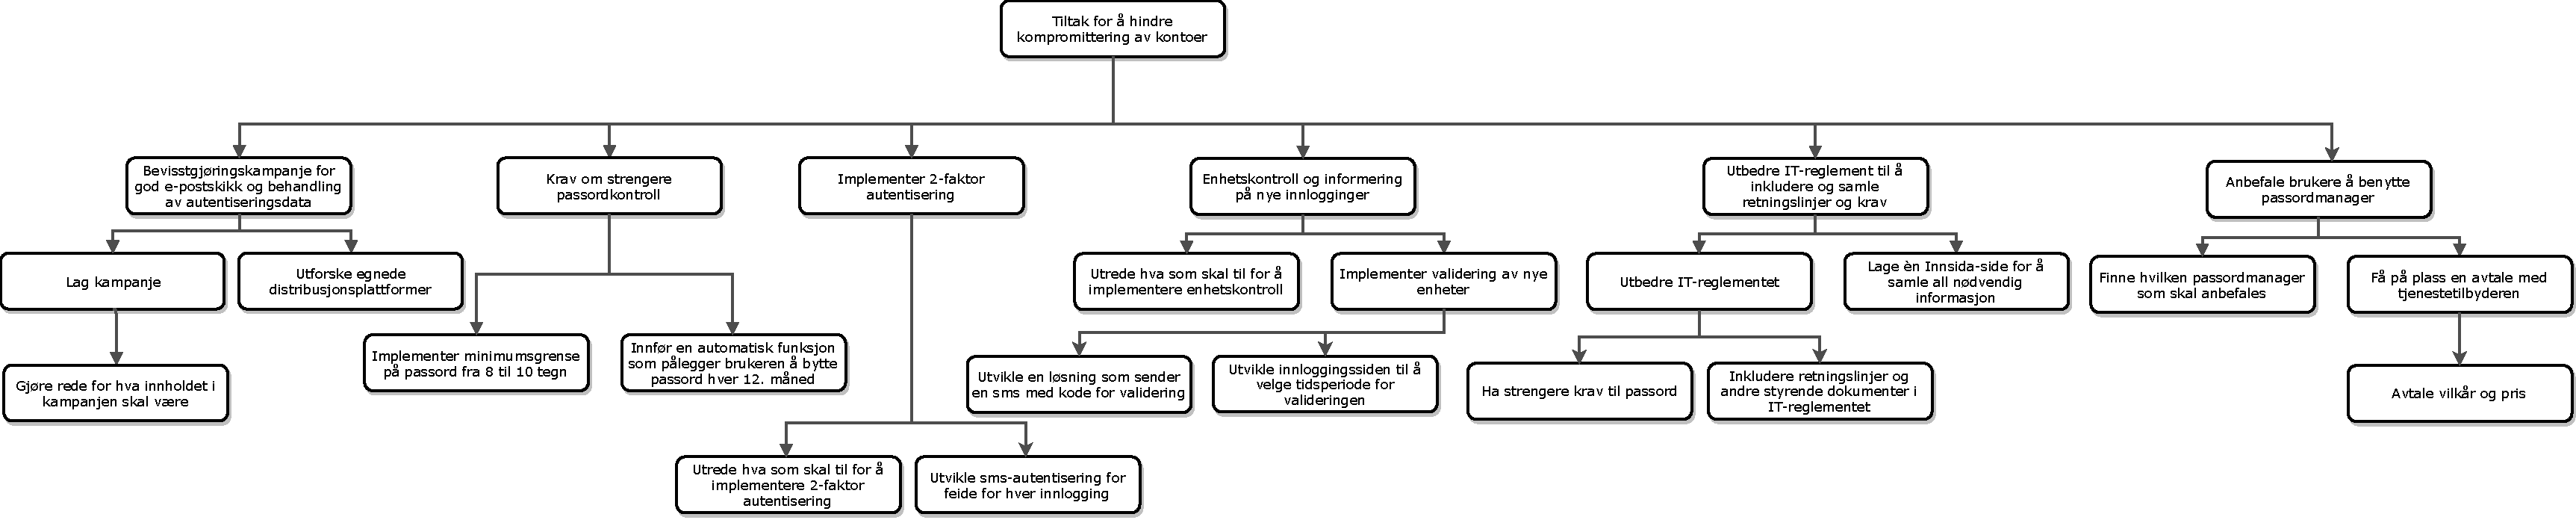
\includegraphics[scale=0.4, angle=90]{case_2/bilder/trediagram.pdf}
    \caption[Trediagram av tiltak case 2]{Trediagram av tiltak case 2}
    \label{fig:trediagram-case2}
\end{figure}


\subsection{Konklusjon av verktøy}
Dette verktøyet fungerte bra for å lage en plan til hvordan tiltakene skal bli implementert og hva som skal til for at tiltaket blir implementert. Trediagram er god måte å stykke opp arbeidsoppgavene for å skape en visuell prosess med oppgavene som må bli gjort for å nå målet. Det eneste som var problemet var at gruppen vår ikke har tilstrekkelig kunnskap om hvordan noen av tiltakene skal bli implementert.
\chapter{Diskusjon og konklusjon}
Dette kapittelet eksisterer for å reflektere litt over prosessen og resultatene vi kom fram til. Vi vil også diskutere effekten ved bruk av rotårsaksanalyse til å løse informasjonssikkerhetsrelaterte hendelser knyttet til kompromitterte kontoer.

\section{Diskusjon}

1
\section{Konklusjon}


\section{Tidsbruk}


\section{Videre arbeid}
Undersøke hele NTNU, passordvaner, e-post, kjennskap til retningslinjer osv. 

\bibliographystyle{ntnuthesis/ntnubachelorthesis}
\bibliography{case_2/bibliografi}

\appendix %after this line all chapters will have leters instead of numbers
\chapter*{Vedlegg A: }

\end{document}